% Opcje klasy 'iithesis' opisane sa w komentarzach w pliku klasy. Za ich pomoca
% ustawia sie przede wszystkim jezyk oraz rodzaj (lic/inz/mgr) pracy.
\documentclass[shortabstract]{iithesis}

\usepackage[utf8]{inputenc}
\usepackage{minted}
\usepackage{pifont}
\usepackage{graphicx}
\usepackage{caption}
\usepackage[T1]{fontenc}
\usepackage{lmodern}
\graphicspath{ {./images/} }

%%%%% DANE DO STRONY TYTUŁOWEJ
% Niezaleznie od jezyka pracy wybranego w opcjach klasy, tytul i streszczenie
% pracy nalezy podac zarowno w jezyku polskim, jak i angielskim.
% Pamietaj o madrym (zgodnym z logicznym rozbiorem zdania oraz estetyka) recznym
% zlamaniu wierszy w temacie pracy, zwlaszcza tego w jezyku pracy. Uzyj do tego
% polecenia \fmlinebreak.
\polishtitle    {Infrastruktura czasu i profilowania jądra systemu operacyjnego Mimiker\fmlinebreak}
\englishtitle   {The infrastructure for time and kernel profiling for Mimiker operating system}
\polishabstract {
W każdym szybko rozwijającym się systemie takim jak Mimiker, pojawia się potrzeba optymalizacji.
Do tego niezbędne jest odpowiednie narzędzie mierzące jego wydajność. 
Przedstawię swoją implementację takiego narzędzia dla systemu Mimiker, przy okazji opisując metody zbierania informacji oraz przykładowe profilery.
Praca przybliży infrastrukturę czasu, która jest kluczowa dla poprawnego funkcjonowania profilerów.
Opiszę również dodane przeze mnie funkcjonalności związane z czasem.
}
\englishabstract{
In every fast-growing system like Mimiker, there comes the need to optimize it.  To do so, you need the right tool to measure the system's performance.
I will present the implementation of such a tool for the Mimiker system. Moreover, I will describe the methods of collecting information and examples of profiles.
The work will also introduce the time infrastructure, which is crucial for profilers.
I will also describe the time functionalities which I implemented.
}
% w pracach wielu autorow nazwiska mozna oddzielic poleceniem \and
\author         {Wiktor Pilarczyk}
% w przypadku kilku promotorow, lub koniecznosci podania ich afiliacji, linie
% w ponizszym poleceniu mozna zlamac poleceniem \fmlinebreak
\advisor        {Krystian Bacławski, Piotr Witkowski}
%\date          {}                     % Data zlozenia pracy
% Dane do oswiadczenia o autorskim wykonaniu
%\transcriptnum {}                     % Numer indeksu
%\advisorgen    {dr. Jana Kowalskiego} % Nazwisko promotora w dopelniaczu
%%%%%

%%%%% WLASNE DODATKOWE PAKIETY
%
%\usepackage{graphicx,listings,amsmath,amssymb,amsthm,amsfonts,tikz}
%
%%%%% WŁASNE DEFINICJE I POLECENIA
%
%\theoremstyle{definition} \newtheorem{definition}{Definition}[chapter]
%\theoremstyle{remark} \newtheorem{remark}[definition]{Observation}
%\theoremstyle{plain} \newtheorem{theorem}[definition]{Theorem}
%\theoremstyle{plain} \newtheorem{lemma}[definition]{Lemma}
%\renewcommand \qedsymbol {\ensuremath{\square}}
% ...
%%%%%

\usepackage{amsthm, listings, epigraph}

\theoremstyle{definition} \newtheorem*{definition}{Definicja}
\theoremstyle{definition} \newtheorem*{example}{Przykład}
\theoremstyle{definition} \newtheorem*{remark}{Uwaga}

\setminted{
    autogobble,
}
\newenvironment{longlisting}{\captionsetup{type=listing}}{}

\lstset{
    basicstyle=\ttfamily\small,
    numberstyle=\footnotesize,
    numbers=left,
    frame=single,
    extendedchars=true,
    literate={ą}{{\k{a}}}1 {Ą}{{\k{A}}}1 {ę}{{\k{e}}}1 {Ę}{{\k{E}}}1 {ó}{{\'o}}1 {Ó}{{\'O}}1 {ś}{{\'s}}1 {Ś}{{\'S}}1
             {ł}{{\l{}}}1 {Ł}{{\L{}}}1 {ż}{{\.z}}1 {Ż}{{\.Z}}1 {ź}{{\'z}}1 {Ź}{{\'Z}}1 {ć}{{\'c}}1 {Ć}{{\'C}}1
             {ń}{{\'n}}1 {Ń}{{\'N}}1
}

\makeatletter
\AtBeginDocument{%
  \newcounter{llabel}[listing]%
  \renewcommand*{\thellabel}{%
    \ifnum\value{llabel}<0 %
      \@ctrerr
    \else
      \ifnum\value{llabel}>10 %
        \@ctrerr
      \else
        \protect\ding{\the\numexpr\value{llabel}+201\relax}%
      \fi
    \fi
  }%
}
\newlength{\llabelsep}
\setlength{\llabelsep}{1pt}
\newcommand*{\llabel}[1]{%
  \begingroup
  \refstepcounter{llabel}%
  \label{#1}%
  \llap{\thellabel\kern\llabelsep}%
  \endgroup
}
\makeatother

\setminted[c]{escapeinside=@@}

\begin{document}

%%%%% POCZĄTEK ZASADNICZEGO TEKSTU PRACY

\chapter{Wprowadzenie}

Pod koniec zeszłego wieku moc komputerów, a także ich pamięć była znacząco ograniczona. W związku z tym programiści starali się, aby ich programy były jak najlepiej zoptymalizowane. Powstawało wiele ,,sztuczek", które umożliwiały obliczyć tą samą rzecz znacznie mniejszym kosztem. Jedną z najbardziej znanych jest szybka odwrotność pierwiastka kwadratowego \cite{bib:fisr}, rozpowszechniona przez implementację z gry Quake III: Arena. Metoda ta była wykorzystywana do obliczania kątów padania i odbicia np. światła. Sposób ten wykorzystuje właściwości reprezentacji liczby zmiennoprzecinkowej, ale obliczenia dokonuje na reprezentacji liczby całkowitej, co pozwoliło na uniknięcie czasochłonnych operacji zmiennoprzecinkowych.

Wydawać by się mogło, że w obecnych czasach, gdzie dostęp do zasobów obliczeniowych (prawo Moore'a) i pamięciowych (chmura) jest znacząco łatwiejszy, problem optymalizacji zszedł na dalszy tor. Nic bardziej mylnego, wraz z większymi możliwościami wzrosły także zapotrzebowania - wzrost przetwarzanych danych, większe systemy, większa liczba użytkowników, a także podstawowe ekonomiczne podejście do efektywnego korzystania z dostępnych zasobów. Optymalizacje okazują się kluczowe w procesie testowania produktu, gdzie funkcje lub komponenty są testowane wielokrotnie pod względem poprawności, a także sprawności działania. 

Aby mieć możliwość efektywnej poprawy wydajności, chcemy wiedzieć co należy zoptymalizować. Pomijając lokalne usprawnienia, które są często dokonywane przez kompilatory, to zdobycie informacji co należy przyspieszyć nie należy do prostych zadań. Dlatego powstało wiele specjalistycznych narzędzi zbierających odpowiednie informacje pomagające w szukaniu, które fragmenty kodu chcielibyśmy zoptymalizować.

W swojej pracy przedstawię własną implementację narzędzia (o nazwie kgprof)  badającego wydajność jądra systemu Mimiker metodą profilowania, a także opiszę nowe funkcjonalności wprowadzone do infrastruktury czasu w celu m.in.  zapewnienia prawidłowego działania tego narzędzia. Obecny rozdział wprowadza w tematykę badania programów oraz opisuje czym jest system Mimiker. W rozdziale 2 przedstawię infrastrukturę czasu w systemach operacyjnych rodziny BSD, jej kluczowe elementy oraz sposób wykorzystania. Następnie w 3 rozdziale zaprezentuję implementację infrastruktury czasu w systemie Mimiker. Rozdział 4 wprowadza w rodzaje profilowania, narzędzia do analizowania oprogramowania pod względem wydajnościowym, a rozdział 5 opisuje implementację narzędzia kgprof w Mimikerze. W rozdziale 6 podsumowuje swoją prace, a także przedstawię dalsze możliwości rozwoju systemu Mimiker.

\section{Badanie programów}
Narzędzia do badania programu można podzielić ze względu na sposób użycia na analizę statyczną i dynamiczną.

\textbf{Analiza statyczna} polega na analizie kodu bez jego wykonania. Jej wyniki są powtarzalne, ponieważ bazują na samym kodzie, a proces analizy zachodzi w ten sam sposób niezależnie od wywołania. Wykorzystuje się w różnych celach m.in. sprawdzenia składni, spełniania standardów, wykrycia luk w bezpieczeństwie itp.

\textbf{Analiza dynamiczna} bazuje na analizie kodu ze zebranych danych podczas jego wykonywania. Przez to, że dane są zbierane w trakcie wykonywania kodu nie jesteśmy w stanie zagwarantować, że wyniki będą powtarzalne. Podejście to pozwala na przetestowanie oprogramowania pod względem pokrycia kodu, złego zarządzania pamięcią, wydajności itp. Do ostatniego typu należy właśnie profilowanie.

\textbf{Profiler} np. poprzez \textbf{instrumentacje kodu} (dodanie kodu pomocniczego do programu) zbiera informacje podczas jego wykonywania. Zbierane informacje mogą różnić się w zależności od celu profilowania programu. Przykładowo podczas analizowania oprogramowania pod względem pamięciowym zbiera się dane w jakich miejscach jest alokowana pamięć, a także gdzie i kiedy jest wykorzystywana lub zwalniana. Taka analiza oprogramowania pozwala na lepsze wykorzystanie zasobów, a także wykrywanie tzw. wąskich gardeł (ang. bottlenecks).

\section{Projekt Mimiker}

\textbf{Mimiker} jest to projekt naukowy systemu operacyjnego zainspirowanego światem UNIXa z domieszką smaczku *BSD. Głównym jego zadaniem jest rozwój jądra do momentu większego wsparcia dla UNIXowej przestrzeni użytkownika \cite{bib:Mimiker}.

W wyniku ciągłego rozwoju projektu Mimiker, a także rozrastających się jego możliwości niezbędne jest dbanie o bezbłędność oprogramowania. System udostępnia do tego trzy narzędzia do wykrywania nieprawidłowego wykorzystania pamięci (KASAN \cite{bib:kasan}), detekcji wyścigów (KCSAN \cite{bib:kcsan}) lub dynamicznego sprawdzania poprawności kolejności zakładanych blokad (LOCKDEP \cite{bib:lockdep}). Kolejnym podejściem jest testowanie możliwie każdego komponentu pod względem poprawności jego działania. Testy te umożliwiają wczesne wykrycie bugów w przyszłych zmianach. Lepsza weryfikacja systemu poprzez jego testowanie wiąże się z dłuższym działaniem całego procesu dla każdej zmiany. 

Przy rozrastającym się systemie pojawiła się potrzeba narzędzia, które pozwoli poprawić wydajność jądra, a dokładnie umożliwi analizowanie kodu pod tym względem. Takim narzędziem jest właśnie odpowiedni profiler, który potrafi zebrać informacje na temat działania programu oraz ułatwić jego optymalizację. W dalszych rozdziałach opiszę własną implementację profilera (kgprof) jako komponentu jądra systemu Mimiker oraz pokażę w jaki sposób wykorzystuje on funkcjonalności oferowane przez kompilator (instrumentacja kodu) i  debugger (dostęp do struktur danych przestrzeni jądra). Działanie profilera opiera się na próbkowaniu, czyli badaniu stanu systemu w ściśle okreslonych odstępach czasu. Do wyznaczania tych odstępów służą obecne w systemie zegary, które również trzeba oprogramować. Stąd zależność profilowania od infrastruktury czasu, którą także opiszę w tej pracy.

W związku z tym ostatnim zagadnieniem opiszę też zmiany, które umożliwiły ustawienie czasu nieulotnego podczas bootowania systemu, działanie wywołań systemowych gettimeofday i nanosleep, ustandaryzowanie używania struktury bintime\_t w jądrze, usunięcie czasochłonnych operacji modulo podczas odczytu z zegarów czy doprowadzenie do działania zegara PIT. 

Ostatnia funkcjonalność okazała się kluczowa, ponieważ dzięki dwóm sprawnym zegarom w systemie, można asynchronicznie względem zegara systemowego (za pomocą drugiego) próbkować jądro systemu. Jest to o tyle kluczowe, że niektóre programy mogą się zsynchronizować z działaniem zegara systemowego. Przykładowo mogą działać względnie dużą część czasu, ale regularnie przed wywołaniem rutyny kończą wykonanie lub idą spać, przez co nie mamy możliwości ich zaobserwować w ten sposób. Dlatego niezależne zbieranie danych pozwala na lepsze odzwierciedlenie działania systemu. Pozwoli to w pełni korzystać z dodanego przeze mnie do Mimikera profilera kgprof opartego na gprof \cite{bib:gprof}. 

\chapter{Infrastruktura czasu}

\section{Podstawowe pojęcia - rozdzielczość, precyzja i stabilność}

Ważnymi pojęciami do uświadomienia jak działają zegary jest rozdzielczość, precyzja i stabilność \cite{bib:timecounters}. Pojęcia wydawać się mogą podobne, lecz każde z nich opisuje inną właściwość zegara.  \textbf{Rozdzielczość} (ang. resolution) inaczej zwana \textbf{częstotliwością} (ang. frequency) zegara to zakładana średnia liczba tyknięć wykonywanych w przeciągu sekundy. \textbf{Okres} czyli ile trwa przerwa pomiędzy tyknięciami jest odwrotnością częstotliwości, \textbf{precyzja} (ang. precision) opisuje ile średnio różni się okres pomiędzy rzeczywistymi tyknięciami, a podanym, zaś \textbf{stabilność} (ang. stability) określa jak duże są wahania pomiędzy okresami tyknięć. Każdy zegar charakteryzuje się własną specyfikacją i nie mając wiarygodnego źródła odniesienia, nie istnieje skuteczna metoda, aby określić jego parametry. Dlatego jedyną, ale za to podstawową własność jaka powinna być zagwarantowana niezależnie od architektury to, aby mierzony czas płynął do przodu.

\section{Zegary sprzętowe}
W systemach można wyróżnić kilka rodzajów zegarów (liczników) sprzętowych, które różnią się charakterystyką mierzenia czasu, a co za tym idzie także służą do różnych celów. Do najbardziej rozpowszechnionych należą:

\subsection{TSC}
\textbf{Timestamp Counter} (TSC) odnosi się do rejestru występującego w architekturze x86-32 np. Intel Pentium \cite{bib:lpi}. Rejestr ten przechowuje informacje o odbytych cyklach procesora od uruchomienia maszyny.

Rozdzielczość takiego zegara jest bardzo wysoka, ale nie jest ona stała co jest jego główną wadą. W praktyce oznacza to niską stabilności (częstotliwość procesora może się wahać, są też procesory, które umożliwiają zmianę trybu pracy na energooszczędny przez co zmniejszają swoją częstotliwość taktowania \cite{bib:freebsd-os}), a w przypadku wielordzeniowego procesora, gdzie każdy rdzeń może mieć swój licznik pojawia się problem synchronizacji pomiędzy rdzeniami.

Podobne rejestry stosuje się w innych procesorach, lecz są one inaczej nazywane - np. Cycle Counter Register (CCNT) w ARM11 \cite{bib:ccnt}.

\subsection{Zegar programowalny}

\textbf{Zegar programowalny} jak jego nazwa wskazuje umożliwia jego zaprogramowanie (przykładowy licznik to Intel 8254 nazywany też \textbf{PIT} (Programmable Interval Timer)). W zależności od osprzętu zegar może działać w różnych trybach, najpopularniejsze z nich to \textbf{jednostrzałowy} (ang. one-shot), który wysyła sygnał za ustalony czas, a także \textbf{okresowy} (ang. periodic) gdzie sygnał jest wysyłany z ustaloną częstotliwością. 

\subsection{RTC}
\textbf{Real time clock} (RTC) jest to zegar powszechnie stosowany w komputerach, aby mieć możliwość śledzenia czasu podczas gdy maszyna jest wyłączona \cite{bib:lkd}. W porównaniu z poprzednikami ten rodzaj czasomierzu jest nieulotny, czyli posiada zazwyczaj osobne źródło zasilania, które umożliwia śledzenie czasu niezależnie od tego czy maszyna jest uruchomiona.

\section{Reprezentacje czasu}
W systemach operacyjnych poprzez różne zapotrzebowania, a także możliwości powstało wiele sposobów utrzymywania czasu. Jednym z nich jest struktura \textbf{tm}, która dla każdego atrybutu ma oddzielne pole opisujące tą własność, jest to podobny sposób w jaki człowiek odnosi się do przedstawiania czasu - w formie kalendarzowej \cite{bib:tm_t}.

\begin{longlisting}
  \begin{minted}{c}
typedef struct tm {
	int	tm2_sec>:	/* seconds after the minute [0-60] */
	int	tm_min;	/* minutes after the hour [0-59] */
	int	tm_hour;       /* hours since midnight [0-23] */
	int	tm_mday;       /* day of the month [1-31] */
	int	tm_mon;	/* months since January [0-11] */
	int	tm_year;       /* years since 1900 */
	int	tm_wday;       /* days since Sunday [0-6] */
	int	tm_yday;       /* days since January 1 [0-365] */
	int	tm_isdst;      /* Daylight Savings Time flag */
	long       tm_gmtoff;     /* offset from UTC in seconds */
	char       *tm_zone;      /* timezone abbreviation */
    } tm_t;
  \end{minted}
  \caption{\href{https://mimiker.ii.uni.wroc.pl/source/xref/mimiker/include/sys/time.h?r=9505a819\#8}{Struktura tm}}
  \label{lst:structtm}
\end{longlisting}

Do ciekawszych pól tej struktury należą:

\begin{itemize}
    \item \textbf{tm\_isdst} flaga, gdzie dodatnia wartość oznacza, że uwzględnia się czas letni w prezentowanym czasie, zero nie uwzględnia, a negatywna, że informacja nie jest dostępna
    \item \textbf{tm\_gmtoff} liczba sekund, które należy dodać do UTC (opisane poniżej), aby otrzymać czas lokalny przechowywany w tej strukturze
    \item \textbf{tm\_zone} zawiera nazwę strefy czasowej użytej do obliczenia czasu np. 
\end{itemize}

Zaletą takiej reprezentacji jest łatwy dostęp do charakterystyk opisywanych przez pola. Natomiast wadą nieefektywność pamięciowa (większość pamięci jest niewykorzystana), mała precyzja, a także niewydajność (obliczanie różnicy lub porównywanie dat wymaga więcej operacji niż w innych stosowanych strukturach, które są poniżej przedstawione).

W jądrze systemów operacyjnych głównie operuje się na strukturach, które składają się z dwóch pól. Pierwsze pole reprezentuje sekundy, a drugie część ułamkową sekundy (time\_t zazwyczaj jest to 64 bitowa liczba całkowita). Zaletą tego rozwiązania jest prostota, a także duża efektywność. Jedną z takich struktur jest \textbf{timeval}, która operuje na sekundach i mikrosekundach \cite{bib:time-types}.

\begin{longlisting}
  \begin{minted}{c}
    typedef struct timeval {
      time_t tv_sec;       /* seconds */
      suseconds_t tv_usec; /* microseconds */
    } timeval_t;
  \end{minted}
  \caption{\href{https://mimiker.ii.uni.wroc.pl/source/xref/mimiker/include/sys/time.h?r=9505a819\#22}{Struktura timeval}}
  \label{lst:structtv}
\end{longlisting}

Jej nowszym wariantem jest \textbf{timespec}, która różni się tym od poprzednika, że zamiast mikrosekund utrzymuje nanosekundy. Pozwala to na większą dokładność w mierzeniu czas. Powstanie tej struktury wynika z szybko rozwijającej się technologii, która umożliwiła przyspieszenie taktowania procesorów, a to pośrednio przyczyniło się do potrzeby dokładniejszej reprezentacji czasu \cite{bib:time-types}.

\begin{longlisting}
  \begin{minted}{c}
    typedef struct timespec {
      time_t tv_ses; /* seconds */
      long tv_nsec;  /* nanoseconds */
    } timespec_t;
  \end{minted}
  \caption{\href{https://mimiker.ii.uni.wroc.pl/source/xref/mimiker/include/sys/time.h?r=9505a819\#27}{Struktura timespec}}
  \label{lst:structts}
\end{longlisting}

Głównym problemem powyższych reprezentacji jest ich zamkniętość na usprawnienia (zwiększenie częstotliwości zegara lub potrzeba dokładniejszej reprezentacji czasu). Struktura bardziej uniwersalna na rozdzielczość zegara jest \textbf{bintime}. Jak poprzednicy również utrzymuje sekundy i część ułamkową, lecz ułamek jest reprezentowany w systemie dwójkowym, czyli liczba jest przechowywana w postaci \textbf{stało-pozycyjnej}.

\begin{longlisting}
  \begin{minted}{c}
    typedef struct bintime {
     time_t sec;    /* second */
     uint64_t frac; /* a fraction of second */
    } bintime_t;
  \end{minted}
  \caption{\href{https://mimiker.ii.uni.wroc.pl/source/xref/mimiker/include/sys/time.h?r=9505a819\#32}{Struktura bintime}}
  \label{lst:structbt}
\end{longlisting}

\begin{figure}[ht]
\centering
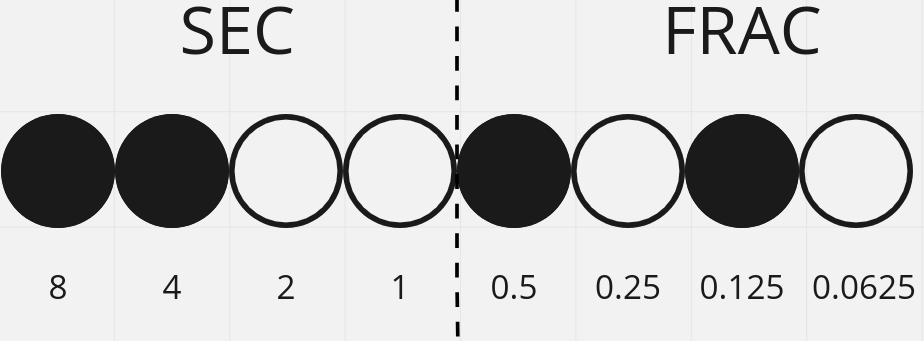
\includegraphics[scale=0.4]{secfrac.png}
\caption{Wizualizacja reprezentacji liczby 12.625 w przypadku kiedy pola sec i frac miałyby tylko 4 bity.}
\end{figure}

Przeznaczenie na część ułamkową sześćdziesięciu czterech bitów pozwala zaspokoić zegary o częstotliwości $1/2^{-64} \approx 1.84 * 10^{19} Hz = 1.84* 10^{10} GHz $ (aktualnie największa częstotliwość osiągnięta przez CPU to $8.42938$ GHz \cite{bib:guinness}). Może pojawić się pytanie czy nie wystarczy przeznaczyć tylko trzydziestu dwóch bitów, aby trzymać część sekundy? Taka forma przedstawienia ułamka jest niewystarczająca, ponieważ ogranicza zegary, których częstotliwość jest większa niż $1/2^{-32} \approx 4.29^{9} Hz = 4.29$ GHz.

\section{Czas EPOCH}
\textbf{Unix EPOCH} zwany też czasem UNIXowym lub POSIXowym. Jest to powszechnie przyjęta konwencja, od którego momentu liczony jest czas w systemach operacyjnych, może być porównany do rozróżniania p.n.e. od n.e. podobnie w komputerach korzysta się z symbolicznej daty - 1 stycznia 1970 00:00:00 UTC \cite{bib:apue}. Początkowo przyjmowano rozpoczęcie odliczania od 1 stycznia 1900 roku, lecz powodowało to problemy gdyż licznik lat zazwyczaj ograniczano od [0-99]. Generowało to problem pojawiający się podczas zmiany wieków pomiędzy rokiem 1999, a 2000 (problem ten występuje np. w zegarze MC146818 RTC, który wykorzystujemy w Mimikerze). Zwany problemem roku 2000 \cite{bib:y2k}, w którym obawiano się potencjalnych skutków związanych z tą reprezentacją czasu w systemach komputerowych. Reprezentacja EPOCH była odporna na tą dotkliwość. Natomiast ta reprezentacja czasu też nie jest bez wad, gdyż podobny problem pojawia się 19 stycznia 2038 03:14:07 UTC dla urządzeń korzystających z 32-bitowej reprezentacji EPOCH. W tym terminie nastąpi przepełnienie dla struktur trzymających sekundy w formie 32-bitowego inta i jeśli systemy nie zapewnią obejścia dla tego problemu to zegary pokażą datę 13 grudnia 1901 20:45:52 UTC. Aktualnie większość maszyn pracuje na 64 bitowej architekturze i ten problem nie występuje.

\subsubsection{UTC}

\textbf{UTC} inaczej uniwersalny czas koordynowany (ang. Universal Time Coordinated) \cite{bib:utc} jest to międzynarodowy standard do wyznaczania czasu do celów cywilnych i naukowych, stworzony do dostosowywania się czasu atomowego względem słonecznego, który nie jest stabilny w związku z fluktuacjami rotacji Ziemi. Główną motywacją tego czasu jest, aby Słońce średnio przechodziło nad południkiem zerowym o godz. 12:00 UTC. Do synchronizacji czasu wykorzystuje się sekundy przestępne.

\subsubsection{Sekunda przestępna}
Nazywana też \textbf{sekundą skokową}, która jest okazjonalnie dodawana (może być też odjęta, ale nie było takiego przypadku) do precyzyjnie mierzonego czasu (np. przez zegary atomowe). Przykładowo trzydziestego pierwszego grudnia 2016, po upływie sekundy o godzinie 23:59:59 nastąpiła 23:59:60, zamiast 00:00:00. Do dnia 1 stycznia 2021 dodano łącznie 27 sekund przestępnych.

Reprezentacja ta (EPOCH) sama w sobie nie uwzględnia sekund skokowych, których nie można przewidzieć \cite{bib:leapsec}. Przez co reprezentacja (bez odpowiedniej synchronizacji) wyprzedza rzeczywisty czas o sekundy przestępne, które upłynęły. W komputerach, które są podłączone do sieci internetowej wykorzystuje się protokół \textbf{NTP} \cite{bib:unp} do synchronizacji czasu, co w szczególności uwzględnia sekundy przestępne.

\section{Rutyny na podstawie systemów *BSD}
\textbf{Rutyny} to funkcje, których wołanie jest powtarzalne, zazwyczaj co pewien stały okres. Postaram się przybliżyć najważniejsze zadania jakie należą do nich.

W systemach *BSD rutyny są kluczowymi funkcjami umożliwiającymi sprawne działanie jądra - m.in. odpowiadają za aktualizację czasu czy umożliwiają obliczanie priorytetów dla planowania procesów.

Są dwa główne podejścia do zarządzania rutynami:

\begin{itemize}
    \item system stara się dla każdej z rutyn przydzielić osobny zegar w trybie okresowym, aby były od siebie niezależne. W przypadku kiedy nie można przydzielić osobnego zegara główna rutyna obsługuje mniejsze - rozwiązanie stosowane w systemie NetBSD lub Mimiker
    \item system  korzysta tylko z jednego zegara w trybie jednostrzałowym i obsługuje rutyny, którym termin minął, a następnie oblicza, która rutyna ma zostać wykonana najwcześniej i planuje przerwanie na ten moment - sposób zarządzania rutynami we FreeBSD
\end{itemize}

Czyli z perspektywy zegara jedno podejście z góry określa, że funkcja będzie wywoływana co pewien okres, zaś druga po obsłużeniu odpowiedniej/ich rutyn odpowiada na pytanie za ile należy obsłużyć następną rutynę, a następnie ustawia termin dla zegara w trybie jednostrzałowym. 

Pierwszy sposób pozwala na łatwiejszą manipulację rutyną, ponieważ każda rutyny ma swój zegar o ile to możliwe, a także rutyny mogą być obsługiwane współbieżnie. Zaś drugie podejście wiąże się z delikatnie większym narzutem, ponieważ za każdym razem chcemy ustawić zegar, ale za to potrzebuje tylko jednego zegara.

Przedstawię funkcje wykorzystywane we FreeBSD. W systemie tym znajdziemy trzy główne rutyny:

\begin{itemize}
    \item \textbf{hardclock} głównym zadaniem jest aktualizacja czasu
    \item \textbf{statclock} prowadzi statystyki dla procesu
    \item \textbf{profclock} zbiera informacje o wydajności procesu
\end{itemize}

Warto zwrócić uwagę, że rutyny pomiędzy systemami *BSD są bardzo podobne, ale zawierają między sobą drobne różnice np. w systemie NetBSD zadania funkcji profclock są obsługiwane przez funkcję statclock.

Do wywoływania tych rutyn wykorzystuje się mechanizm \textbf{przerwań zegarowych}, które za pomocą zegara w zaplanowanym momencie wywołują funkcję, która obsługuje powyższe rutyny.

\subsubsection{Przerwanie}
Zewnętrzny sygnał, który niezależnie od aktualnie wykonywającego się procesu (z wyjątkiem procesów, które obsługują przerwanie) powoduje jego zatrzymanie i zmianę przepływu sterowania. Przerwania mogą mieć różne priorytety (obsługa przerwania o niższym priorytecie może być wstrzymana poprzez przerwanie o wyższym priorytecie).

Interwał, z jaką dokładnością aktualizuje się czas nazywany jest \textbf{tyknięciem systemowym} (zazwyczaj częstotliwość wynosi 1000 Hz). Czasami system nie potrzebuje, aby tyknięcia zachodziły tak często (np. laptop w trybie uśpienia), wtedy takie przerwanie jest odwlekane. Sposób ten pozwala na oszczędzanie baterii w laptopach czy telefonach. Funkcja obsługująca to przerwanie jest \textbf{hardclock}.

\subsection{Hardclock}

Nazwa wzięła się od połączenia hardware i clock, ponieważ zegar ten zawsze był związany z zegarem fizycznym.

Funkcja wołana jest podczas przerwania zegarowego i jej zadaniami \cite{bib:freebsd-os} są:

\begin{itemize}
    \item aktualizowanie czasu (opisany poniżej) i wdrażanie poprawek do czasu (wynikające z protkołu NTP opisanego poniżej)
    \item aktualizowanie wirtualnych zegarów (zegary, które udostępniają funkcjonalności jak zegary fizyczne, ale w rzeczywistości opierają się na zegarze fizycznym, zazwyczaj jednym)
\end{itemize} 

Ważne, aby czas działania hardclocka  nie był dłuższy niż tyknięcie systemu, ponieważ przerwanie zegarowe, ma na tyle wysoki priorytet, że może nastąpić głodzenie innych procesów.

\subsubsection{NTP}

\textbf{Network time protocol} protokół sieciowy wykorzystywany do synchronizacja czasu pomiędzy komputerami (z dokładnością do milisekund) \cite{bib:unp}. Podczas aktualizacji czasu w hardclocku koryguje się jego wskazania, z informacji uzyskanych dzięki protokołowi.

\subsection{Statclock i profclock}

We wcześniejszych wersjach FreeBSD hardclock zajmował się zbieraniem informacji na temat działania systemu, na podstawie którego obliczano przyszłe priorytety w schedulerze. Pojawia się wyżej opisany problem,  przy tym rozwiązaniu procesy mogą się zsynchronizować z tyknięciem systemowym przez co zebrane dane mogłyby nie odzwierciedlać rzeczywistego zużycia zasobów.

Obecnie korzysta się ze \textbf{statclocka} (od ang. statistic) (z częstotliwością 127 Hz \cite{bib:freebsd-os}), który aktualizuje informacje o wykorzystywanych zasobach (np. wykorzystywanej pamięci) i nalicza tyknięcia działającemu wątkowi, a następnie woła scheduler do przeliczania priorytetu (opisane poniżej).

Dodatkowym narzędziem do zbierania informacji jest \textbf{profclock} (od ang. profiling)  (z częstotliwością 1024 Hz \cite{bib:freebsd-os}), który służy do profilowania danego procesu, wykorzystywany np. przez gprofa.

\subsection{Aktualizacja i odczyt czasu}

Nie wszystkie zegary zapewniają atomowość odczytu czasu, ponieważ zazwyczaj najpierw należy pobrać wartość licznika (w niektórych licznikach wymaga to np. dwóch osobnych operacji), a następnie przekonwertowania liczby tyknięć do odpowiedniej reprezentacji czasu. Innym problemem jest zbyt mały rozmiar licznika, który nie chroni przed częstym występowaniem nadmiaru. Z tego powodu wynika potrzeba synchronizacji pomiędzy odczytem ze struktury przechowującej czas, a zaktualizowaniem jej z odczytem z zegara. Wydawać by się mogło, że najłatwiejszym rozwiązaniem jest zastosowanie mechanizmu blokad czytelnik-pisarz \cite{bib:rwlock}, ale aktualizacja zegara występuje pod przerwaniem, więc w przypadku kiedy wywłaszczyliśmy czytelnika trzymającego blokadę, może wystąpić zakleszczenie (ang. deadlock). W prostszych systemach korzysta się ze zwykłych blokad wirujących, ale jest to związane z dodatkowym obciążeniem, które wynika z ich zakładaniem, a aktualizacja czasu jest na tyle częstą rutyną przez co proces ten nie jest optymalny. Jednym z rozwiązań stosowanych w systemach operacyjnych *BSD jest struktura pierścienia, która przechowuje informacje o czasie z możliwym minimalnym opóźnieniem, ale podejście to pozwala na wyeliminowanie blokad \cite{bib:timecounters}.

Pierścień jest cykliczną listą jednokierunkową składającą się z segmentów, które są aktualizowane tylko poprzez jedną rutynę (edytor) (jeden proces naraz może modyfikować strukturę), lecz może występować wiele procesów, które chcą dokonywać odczytu czasu. Edytor za pomocą round-robina aktualizuje kolejne segmenty. Podczas edytowania takiego segmentu najpierw oznacza, że jest zmieniany, następnie aktualizuje czas, a pod koniec zwiększa wersje segmentu. Czytelnik zaś najpierw odczytuje wersje segmentu, następnie pobiera czas, a pod koniec jeśli wersja się zmieniła lub segment jest aktualizowany ponawia całą procedurę, aby otrzymać spójne dane.

Na podstawie implementacji w NetBSD \cite{bib:netbsdtime} omówię proces aktualizacji czasu i dostępu do niego.

\begin{longlisting}
  \begin{minted}{c}
struct timehands {
	struct bintime       th_offset;        /* bin (up)time at windup */
	/* ... */
	volatile u_int       th_generation;    /* current genration */
	struct timehands     *th_next;         /* next timehand */
};
  \end{minted}
  \caption{\href{http://bxr.su/NetBSD/sys/kern/kern_tc.c\#95}{Fragment struktury timehands w NetBSD}}
  \label{lst:structth}
\end{longlisting}

\begin{longlisting}
  \begin{minted}{c}
/*
 * Initialize the next struct timehands in the ring and make
 * it the active timehands.
 */
static void
tc_windup(void)
{
	struct timehands *th, *tho;
	u_int ogen;

	/*
	 * Make the next timehands a copy of the current one, but do not
	 * overwrite the generation or next pointer.  While we update
	 * the contents, the generation must be zero.
	 */
	tho = timehands;
	th = tho->th_next;
	ogen = th->th_generation;
	@\llabel{generation}@th->th_generation = 0;

	th->th_offset += time_since_last_windup();

	/*
	 * Now that the struct timehands is again consistent, set the new
	 * generation number, making sure to not make it zero.
	 */
	@\llabel{ogen}@if (++ogen == 0)
		ogen = 1;
	th->th_generation = ogen;

	/*
	 * Go live with the new struct timehands.
	 */
	@\llabel{timehands}@timehands = th;

	/*
	 * Force users of the old timehand to move on.  This is
	 * necessary for MP systems; we need to ensure that the
	 * consumers will move away from the old timehand before
	 * we begin +updating it again when we eventually wrap
	 * around.
	 */
	if (++tho->th_generation == 0)
		tho->th_generation = 1;
}
  \end{minted}
  \caption{\href{http://bxr.su/NetBSD/sys/kern/kern_tc.c\#753}{Fragment tc\_windup w NetBSD}}
  \label{lst:functcwind}
\end{longlisting}

Podczas aktualizacji czasu poruszamy się po pierścieniu, gdzie aktualizujemy jego następny fragment. Najpierw oznaczamy, że jest modyfikowany \ref{generation}, następnie aktualizujemy pole z przechowywanym czasem, a także zwiększamy generacje tego fragmentu, co pozwala śledzić aktualność naszych odczytów \ref{ogen}. Na koniec ustawiamy ten fragment jako najbardziej aktualny \ref{timehands}.

\begin{longlisting}
  \begin{minted}{c}
void
getbinuptime(struct bintime *bt)
{
	struct timehands *th;
	u_int gen;
    /* ... */
	do {
		th = timehands;
		gen = th->th_generation;
		*bt = th->th_offset;
	@\llabel{gen0}@} while (gen == 0 || gen != th->th_generation);
}
  \end{minted}
  \caption{\href{http://bxr.su/NetBSD/sys/kern/kern_tc.c\#417}{Fragment getbinuptime w NetBSD}}
  \label{lst:funcgetbin}
\end{longlisting}

Podejście to pozwala na atomowy odczyt czasu bez wyłączania przerwań lub stosowania blokad. Odczyt może się nie udać \ref{gen0} w przypadku, kiedy aktualny fragment pierścienia jest aktualizowany (nasza maszyna może być wieloprocesorowa, więc podczas odczytu może odbywać się aktualizacja segmentu) lub jeśli fragment naszego pierścienia został zaktualizowany, a my nie zdążyliśmy w tym czasie zrobić odczytu (bo np. zostaliśmy wywłaszczeni). 

\section{Przetwarzanie opóźnień}

\textbf{Callouty} są wykorzystywane, aby wywołać daną funkcję o konkretnym czasie w przyszłości \cite{bib:calloutbsd}. Ciekawy jest sposób w jaki te wydarzenia są przechowywane. Mamy pewną ograniczoną liczbę kubełków, do których trafiają zadania. Wybór kubełka zależy od obliczonego hasza dla wydarzenia. Kluczem do obliczenia hasza jest termin zadania, a sam hasz wylicza się obliczając modulo po liczbie kubełków. Każdy kubełek przechowuje kolejkę zadań o tym samym haszu. Każde wywołanie callout\_process przechodzi do kubełka o wyższym indeksie (jeśli takiego nie ma przechodzi do pierwszego kubełka), czasami może być to więcej kubełków jeśli upłyneło odpowiednio dużo czasu. Następnie przechodzi listę zadań w kubełku i jeśli termin wydarzenia upłynął (jest mniejszy od argumentu now) oznaczamy, że należy je wykonać i usuwamy z listy. Reprezentacja ta nazywana jest kolejką kalendarzową (ang. calendar queue) \cite{bib:callendarqueue}.

\begin{figure}[ht]
\centering
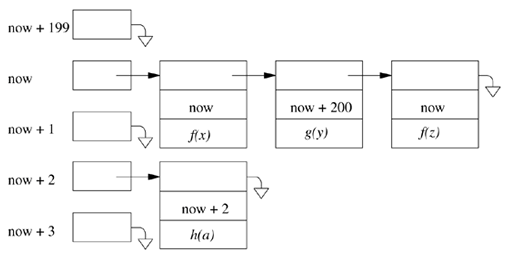
\includegraphics[scale=0.7]{images/callout.png}
\caption{Zilustrowanie działania kubełków, gdzie now symbolizuje aktualną kolejkę i jej 'czas' \cite{bib:freebsd-os}}
\end{figure} 

Podział na kubełki pozwala na średnie przyspieszenie działania kontroli nad terminami, ponieważ nie przegląda się wszystkich elementów, które są zaplanowane, a koszt związany z opóźnionym wykonaniem zadania jest bardzo mały.

\section{Scheduler ULE}

Jednym z kluczowych użytkowników infrastruktury czasu jest scheduler, którego zadaniem jest zarządzanie dostępem do czasu procesora dla wątków. Zazwyczaj dostęp ten jest oparty na zebranych statystykach podczas wcześniej omawianych rutyn (np. stat\_clock).

W systemie FreeBSD występują dwa schedulery jednym z nich jest właśnie ULE \cite{bib:ule}, który powstał wraz z wprowadzeniem rosnącego wsparcia dla SMP (ang. Symmetric MultiProcessing) czyli wykorzystywania jednoczesnego wielu procesorów w jądrze FreeBSD. Poprzedni scheduler 4.4BSD \cite{bib:4bsd-sched} nie skalował się tak dobrze przy wielu CPU.

Skupimy się na mechanizmach związanych z czasem dla procesów współdzielących czas (system zachowuje się inaczej dla wątków obsługujących przerwania lub procesów czasu rzeczywistego).

Pierwszym pojęciem jest \textbf{kwant czasu} dostępu do procesora, który każdy proces dostaje i może wykorzystać. Jeśli będzie działał dłużej zostanie wywłaszczony -- zostanie zażądana zmiana kontekstu z flagą informującą o wykorzystanym czasie. Czas jest naliczany podczas statclocka. W przypadku kiedy proces dobrowolnie poszedł spać resetuje to jego kwant, ponieważ oddał swój możliwy czas na procesorze.

Drugim mechanizmem jest obliczanie priorytetów, a dokładnie stopnia interaktywności dla wątków, aby wiedzieć, który proces należy następnie obudzić. Pozwala to rozróżnić zadania, które wymagają częstszej obsługi (np. terminal zamiast wątku renderującego film).

Do tego wykorzystuje się dwa parametry -- czas działania i czas snu, które w uproszczeniu stanowią sumę czasu spędzonego na procesorze oraz czasu spania naszego procesu. Aby przykładowo długi czas działania programu na początku nie definiował znacząco przyszłego obliczanego priorytetu skaluje się poprzednią sumę (czyli zmniejsza wagę tamtego czasu) przykładowo dzieląc ją przez dwa co jakiś czas, jest to potrzebne, ponieważ wątki mogą zmieniać swój sposób działania. Preferujemy procesy, które mają dłuższy czas spania, ponieważ dobrowolnie oddają swój dostęp do procesora innym procesom, zaś czas działania wpływa negatywnie na priorytet procesu, gdyż korzystając z procesora uniemożliwia innym procesom dostęp do niego.

Podczas analizy funkcji obliczającej priorytet zauważyłem niespójność pomiędzy opisem, a kodem  \cite{bib:ulepr}. Błąd pojawił się także w artykule przedstawiającym ten scheduler \cite{bib:ule} czy też w książce przedstawiającej kluczowe idee systemu FreeBSD \cite{bib:freebsd-os}. Według tego opisu wykres priorytetu wyglądał następująco:

\begin{figure}[H]
\centering
  \centering
  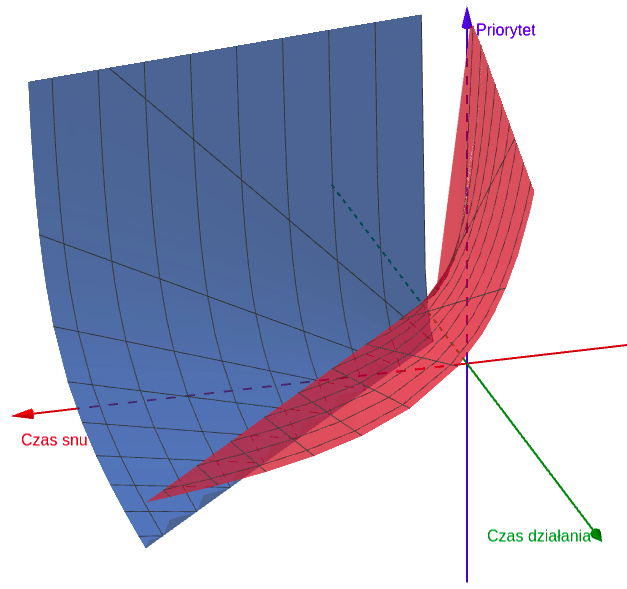
\includegraphics[width=.48\linewidth]{images/ule1.png}
  \label{fig:ule1}
  \centering
  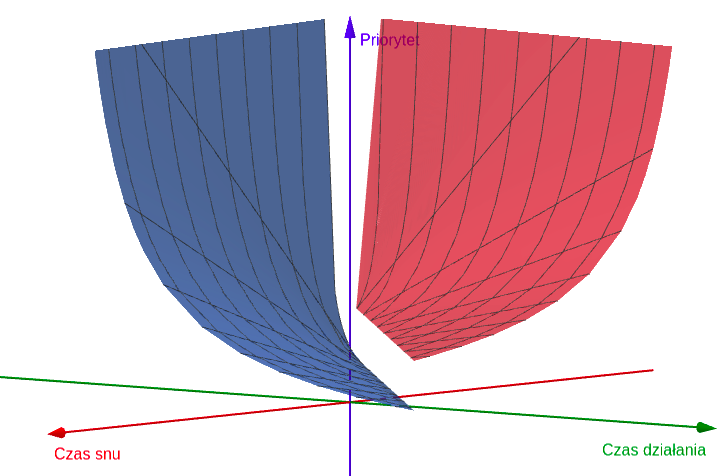
\includegraphics[width=.49 \linewidth]{images/ule2.png}
  \label{fig:ule2}
\caption{Nieprawidłowe wartości funkcji, w zależności od czasu spania i czasu działania}
\label{fig:ule11}
\end{figure}

Widać, że funkcja jest niespójna, a także teoretycznie proces miałby większy priorytet gdyby funkcja cały czas działała i nie spała, niż gdyby działała i trochę spała.
Rzeczywisty wykres prezentuje się następująco:

\begin{figure}[H]
\centering
  \centering
  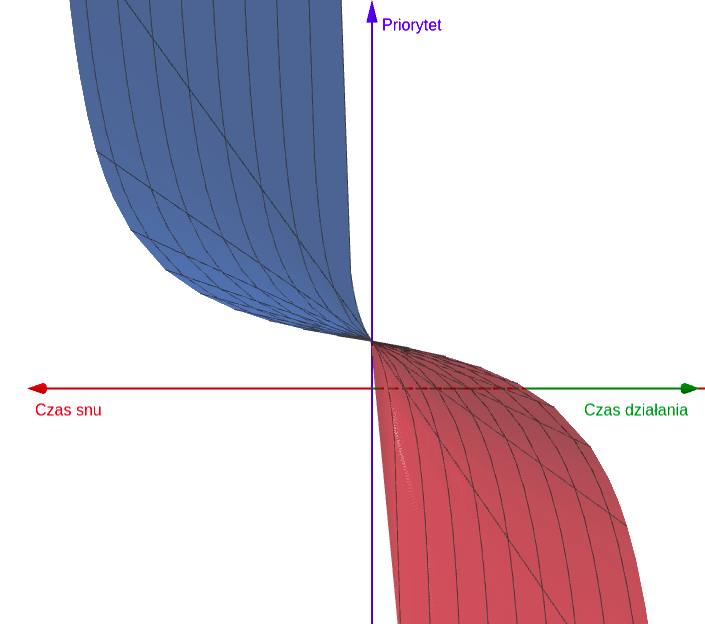
\includegraphics[width=.5\linewidth]{images/sigmoid1.png}
  \label{fig:sig1}
  \centering
  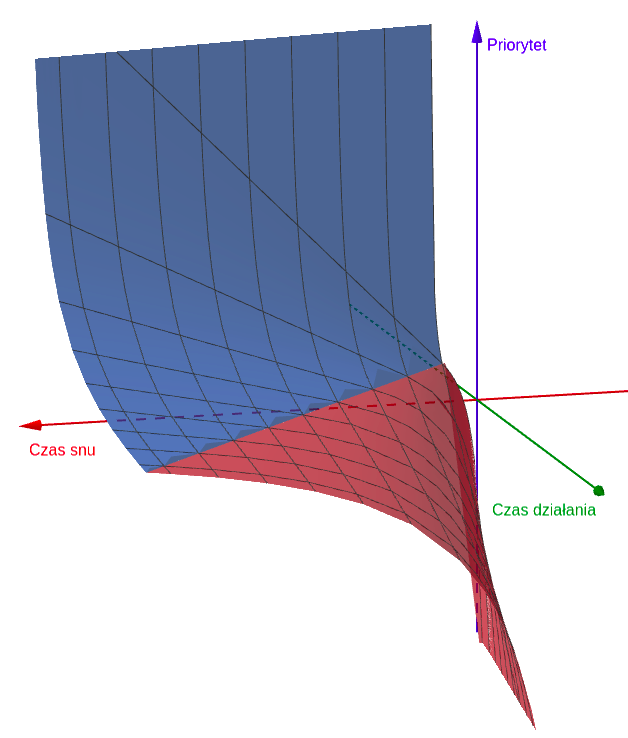
\includegraphics[width=.45 \linewidth]{images/sigmoid2.png}
  \label{fig:sig2}
\caption{Prawidłowe wartości funkcji, w zależności od czasu snu i czasu działania}
\label{fig:sig22}
\end{figure}

Przygotowana przeze mnie zmiana zawierająca poprawę opisu funkcji została zaakceptowana przez programistów rozwijających jądro systemu FreeBSD i wprowadzona do jego kodu \cite{bib:ulepr}.

\chapter{Infrastruktura czasu w Mimikerze}
W systemie Mimiker mamy wsparcie dla dwóch architektur - AArch64 oraz MIPSowej. W przypadku tej pierwszej aktualnie umożliwiamy tylko dostęp do jednego zegara typu TSC -- znajduje się przy procesorze, dlatego skupimy się na tej drugiej, aby móc lepiej zobrazować system.

Wcześniej w jądrze korzystaliśmy z wielu struktur reprezentujących czas. Po wprowadzonych przeze mnie zmianach tam gdzie to możliwe korzystamy z reprezentacji bintime\_t z wcześniej wymienionych powodów (dokładność i skalowalność). Z powodu standardów panujących przy wywołaniach systemowych (m.in. POSIX) nie jest to jedyna struktura, którą stosujemy. Stosowanie się do standardów jest o tyle ważne, że dzięki ujednoliconym zasadom łatwiej jest portować programy z przestrzeni użytkownika pomiędzy systemami.


\section{Zegary sprzętowe}
Zegary sprzętowe są reprezentowane za pomocą specjalnej struktury \textbf{timer\_t}.

\subsection{Struktura timer\_t}
\begin{longlisting}
  \begin{minted}{c}
typedef struct timer {
  TAILQ_ENTRY(timer) tm_link; /*!< entry on list of all timers */
  const char *tm_name;        /*!< name of the timer */
  unsigned tm_flags;          /*!< TMF_* flags */
  unsigned tm_quality;        /*!< how dependable the timer is */
  uint32_t tm_frequency;      /*!< base frequency of the timer */
  bintime_t tm_min_period;    /*!< valid only for TMF_PERIODIC */
  bintime_t tm_max_period;    /*!< same as above */
  tm_start_t tm_start;        /*!< makes timer operational */
  tm_stop_t tm_stop;          /*!< ceases timer from generating new events */
  tm_event_cb_t tm_event_cb;  /*!< callback called when timer triggers */
  tm_gettime_t tm_gettime;    /*!< fetches current time from the timer */
  void *tm_arg;               /*!< an argument for callback */
  void *tm_priv;              /*!< private data (usually device_t *) */
} timer_t;
  \end{minted}
  \caption{\href{https://mimiker.ii.uni.wroc.pl/source/xref/mimiker/include/sys/timer.h?r=4b37e316\#42}{Struktura timer\_t}}
  \label{lst:structtimer}
\end{longlisting}

Pola opisujące charakterystykę zegara lub udostępniające abstrakcję do sterowania nim:

\begin{itemize}

\item \textbf{tm\_link} korzysta z listy dwukierunkowej, makro \textbf{TAILQ\_ENTRY(timer)} tworzy  nowy węzeł listy o typie timer \cite{bib:tailq-man} --- umożliwia dostęp do wszystkich dostępnych zegarów w systemie. Pole to jest przydatne podczas wyboru zegara do rutyny np. do odmierzania czasu. 

\item \textbf{tm\_name} przechowuje nazwę zegara

\item \textbf{tm\_flags} przechowuje flagi trybów zegara w jakich zegar może pracować lub czy zegar jest naszym źródłem czasu

\item \textbf{tm\_quality} określa poziom jakości czasomierza w porównaniu do innych, zegar z większą wartością jest preferowany nad zegarem o mniejszej

\item \textbf{tm\_frequency} podstawowa częstotliwość zegara

\item \textbf{tm\_min\_period} i \textbf{tm\_max\_period} definiują zakres okresu jaki może występować pomiędzy tyknięciami w zegarze

\item \textbf{tm\_start} dostęp do funkcji, która za pomocą argumentów ustawia właściwości zegara (tryb pracy, czy jest źródłem czasu, a także okres), a następnie go uruchamia

\item \textbf{tm\_stop} funkcja powstrzymująca zegar od generowania sygnałów

\item \textbf{tm\_event\_cb} funkcja, która jest wołana kiedy zegar wyśle sygnał

\item \textbf{tm\_gettime} funkcja umożliwiająca odczyt czasu z zegara

\item \textbf{tm\_arg} argumenty, które przyjmuje funkcja tm\_event\_cb

\item \textbf{tm\_priv} dane prywatne, zazwyczaj wskaźnik na strukturę przechowującą informacje o urządzeniu
\end{itemize}

Przed podjęciem pracy korzystaliśmy tylko z MIPSowego zegara, zegar RTC błędnie wskazywał czas, a PIT miał problem z mierzeniem czasu.

\subsection{MIPS timer} 
Zegar ten należy do klasy zegarów \textbf{TSC} - zlicza liczbę cykli procesora, ma on częstotliwość około 100 MHz. Jego rejestr ma tylko trzydzieści dwa bity przez co pojawia się problem z przepełnieniem co około 42 sekundy. Zegar ten jest jednostrzałowy, ale na nasze potrzeby korzystamy z niego jak z okresowego, ponieważ podczas obsługi przerwania automatycznie nastawiamy jego następne przerwanie.

\subsubsection{Odczyt czasu z zegara}
Funkcją umożliwiającą odczyt czasu z zegara jest \textbf{mips\_timer\_gettime} 
\begin{longlisting}
  \begin{minted}{c}
typedef struct mips_timer_state {
  uint64_t sec;         /* seconds passed after timer initialization */
  uint32_t cntr_modulo; /* counter since initialization modulo its frequency */
  uint32_t period_cntr; /* number of counter ticks in a period */
  uint32_t last_count_lo;     /* used to detect counter overflow */
  volatile timercntr_t count; /* last written value of counter reg. (64 bits) */
  volatile timercntr_t compare; /* last read value of compare reg. (64 bits) */
  timer_t timer;
  resource_t *irq_res;
} mips_timer_state_t;

/* ... */
  
static bintime_t mips_timer_gettime(timer_t *tm) {
  device_t *dev = tm->tm_priv;
  mips_timer_state_t *state = dev->state;
  uint64_t sec;
  uint32_t ticks;
  @\llabel{intr_mips_gettime}@WITH_INTR_DISABLED {
    read_count(state);
    sec = state->sec;
    ticks = state->cntr_modulo;
  }
  bintime_t bt = bintime_mul(tm->tm_min_period, ticks);
  assert(bt.sec == 0);
  bt.sec = sec;
  return bt;
}
  \end{minted}
  \caption{\href{https://mimiker.ii.uni.wroc.pl/source/xref/mimiker/sys/mips/timer.c?r=db7eaf68\#11}{Funkcja mips\_timer\_gettime} i \href{https://mimiker.ii.uni.wroc.pl/source/xref/mimiker/sys/mips/timer.c?r=db7eaf68&mo=231&fi=11\#11}{struktura mips\_timer\_state}}
  \label{lst:structmipstimerstate}
\end{longlisting}

Korzystając z makra \textbf{WITH\_INTR\_DISABLED} \ref{intr_mips_gettime} wyłączamy przerawnia (aby odczyt czasu nie został przerwany, co mogłoby spowodować niespójność przy odczycie danych). Funkcja \textbf{read\_count} odczytuje dane z rejestru i przetwarza je. Otrzymujemy sekundy, które upłynęły od uruchomienia zegara oraz liczbę tyknięć modulo częstotliwość zegara (ich sumaryczny okres jest mniejszy od sekundy), następnie tyknięcia są konwertowane do reprezentacji bintime\_t, dane sumowane i otrzymujemy czas. który upłynął od uruchomienia zegara.

\subsubsection{Śledzenie czasu}
Rejestr zegara ma tylko trzydzieści dwa bity, co jest powodem, nadmiaru, który pojawia się co około 42 sekundy ($\frac{2^{32}-1}{10^8} \approx 42$). Dlatego przy regularnych odczytach funkcja \textbf{read\_count} dba o to, aby przepełnienie nie wpływało na odczytany czas.

\begin{longlisting}
  \begin{minted}{c}
typedef union {
  /* assume little endian order */
  struct {
    uint32_t lo;
    uint32_t hi;
  };
  uint64_t val;
} timercntr_t;
  \end{minted}
  \caption{\href{https://mimiker.ii.uni.wroc.pl/source/xref/mimiker/include/sys/timer.h?r=4b37e316\#17}{Unia timercntr\_t}}
  \label{lst:uniontimercntr}
\end{longlisting}

Za pomocą unii \textbf{timercntr\_t} sztucznie rozszerza się możliwość utrzymywania czasu do sześćdziesięciu czterech bitów, co pozwala zapobiec przepełnieniu.

\begin{longlisting}
  \begin{minted}{c}
static uint64_t read_count(mips_timer_state_t *state) {
  SCOPED_INTR_DISABLED();
  @\llabel{mipsreg}@state->count.lo = mips32_getcount();

  /* detect hardware counter overflow */
  if (state->count.lo < state->last_count_lo) {
    state->count.hi++;
  }
  @\llabel{mipsmodulo}@state->cntr_modulo += state->count.lo - state->last_count_lo;

  if (state->cntr_modulo >= state->timer.tm_frequency) {
    state->cntr_modulo -= state->timer.tm_frequency;
    state->sec++;
  }
  @\llabel{mipsmodulocheck}@assert(state->cntr_modulo < state->timer.tm_frequency);

  state->last_count_lo = state->count.lo;
  return state->count.val;
}
  \end{minted}
  \caption{\href{https://mimiker.ii.uni.wroc.pl/source/xref/mimiker/sys/mips/timer.c?r=db7eaf68\#28}{Funkcja read\_count}}
  \label{lst:funcreadcount}
\end{longlisting}

Tak jak poprzednio wyłączane są przerwania, lecz tym razem na całą funkcję, aby zapewnić spójność danych (funkcja jest też wołana w innych miejscach). Odczytuje się rejestr licznika \ref{mipsreg} i przypisuje się dolne trzydzieści dwa bity state$\rightarrow$count (struktura timercntr\_t). Jeśli zostanie zauważone przepełnienie (wartość ostatnich odczytanych dolnych bitów jest większa od aktualnych) to inkrementuje górną część bitów. Dodatkowo na bieżąco obliczana jest liczba sekund oraz liczba cykli modulo częstotliwość \ref{mipsmodulo}. Taki sposób pozwala za pomocą dodatkowych obliczeń w funkcji read\_count pozbyć się obliczania modulo z sześćdziesięcio cztero bitowej liczby (operacja ta jest bardzo czasochłonna i usunięcie jej poprawiło działanie systemu) w funkcji mips\_timer\_gettime. Wydawać się może, że w przypadku kiedy \textbf{last\_count\_lo} jest większe od \textbf{count.lo} występuje problem, ponieważ pojawia się niedomiar, ale zmienne są typu unsigned, więc wynikiem będzie wartość, którą należałoby dodać do ostatniego stanu licznika, aby otrzymać aktualny czyli liczba tyknięć, która upłynęła.

Za pomocą \textbf{asercji} w Mimikerze sprawdzamy czy założenia odnośnie działania programu są spełnione. Jeśli taka asercja nie jest spełniona to powoduje widoczną awarię systemu (ang. system crash) z informacją gdzie nastąpiła. W tym przypadku upewniamy się czy modulo zostało poprawnie obliczone \ref{mipsmodulocheck}, a następnie zapisujemy odczytane wartości i zwracamy wynik.

\subsection{RTC}
Kolejnym zegarem jest zegar MC146818 RTC \cite{bib:rtc}, jako jedyny spośród dostępnych zegarów jest on nieulotny (używany do ustawienia czasu bootowania, który będzie omówiony poniżej), pozwala on odmierzać czas z dokładnością do 1 sekundy, ale za to może generować sygnały z częstotliwością do 4 MHz.

\subsubsection{Odczyt czasu}
Za pomocą funkcji \textbf{rtc\_gettime} mamy możliwość odczytu czasu w formacie tm\_t.
\begin{longlisting}
  \begin{minted}{c}
static void rtc_gettime(resource_t *regs, tm_t *t) {
  t->tm_sec = rtc_read(regs, MC_SEC);
  t->tm_min = rtc_read(regs, MC_MIN);
  t->tm_hour = rtc_read(regs, MC_HOUR);
  t->tm_wday = rtc_read(regs, MC_DOW);
  t->tm_mday = rtc_read(regs, MC_DOM);
  t->tm_mon = rtc_read(regs, MC_MONTH) - 1;
  t->tm_year = rtc_read(regs, MC_YEAR) + 100;
}
  \end{minted}
  \caption{\href{https://mimiker.ii.uni.wroc.pl/source/xref/mimiker/sys/drv/rtc.c?r=825ac182\#57}{Funkcja rtc\_gettime}}
  \label{lst:funcrtcgettime}
\end{longlisting}

W przypadku miesięcy odejmowana jest jedynka, aby reprezentować miesiące, które upłynęły (odpowiada to w jaki sposób przechowuje się miesiące w strukturze tm\_t), a w przypadku lat dodaje się sto, ponieważ zegar przechowuje maksymalną wartość 99 dla lat (związane z opisanym powyżej problemem Y2K). 

\subsection{PIT}
W systemie operacyjnym Mimiker korzystamy z zegara Intel 8254 \cite{bib:pit}, który był powszechnie stosowany w komputerach w latach 90, służył on m.in. do odświeżania pamięci DRAM lub obsługi działania głośników komputerowych. Zgodnie z jego rozwinięciem (Programowalny Zegar Okresowy - Programmable Interval Timer) umożliwia on zaprogramowanie sposobu funkcjonowania naszego czasomierza. Konstrukcyjnie składa się z trzech niezależnych szesnastobitowych liczników. Każdy z liczników można ustawić na jeden z sześciu trybów \cite{bib:pit}. W Mimikerze w ramach naszych potrzeb udostępniamy dostęp tylko do jednego licznika wraz z trybem okresowym.

Zegar ten charakteryzuje się częstotliwością wynoszącą 10MHz, a także wysoką stabilnością. 

Aby utrzymać czas rzeczywisty przez zegar korzystamy z jego trybu okresowego (sprzętowo nazywanego generatorem częstotliwości - \textbf{TIMER\_RATEGEN}), lecz pojawia się problem zgubienia tyknięcia zegara, czyli pominięcia przynajmniej jednego całego okresu.

Wydawać by się mogło, że tak jak poprzednio chcemy porównywać ile tyknięć upłynęło od poprzedniego mierzenia czasu, ale licznik ten jest dużo mniejszy (szesnastobitowy). Dodatkowo nie przechowuje wartości większych niż nadana mu częstotliwość, czyli jeśli maksymalnie może mierzyć okres o długości x tyknięć, to jak ustawimy okres o połowę tyknięć, to maksymalną wartość licznika też zmniejsza się o połowę. Wynika to z tego, że zegar liczy od zera do liczby tyknięć potrzebnych do uzyskania żądanego okresu, wywołuje przerwanie i powtarza proces (sprzętowo licznik ten liczy w dół, ale za pomocą prostego odejmowania liczby tyknięć zegara od okresu w formie tyknięć, korzystamy z licznika w formie rosnącej).

\begin{figure}[ht]
\centering
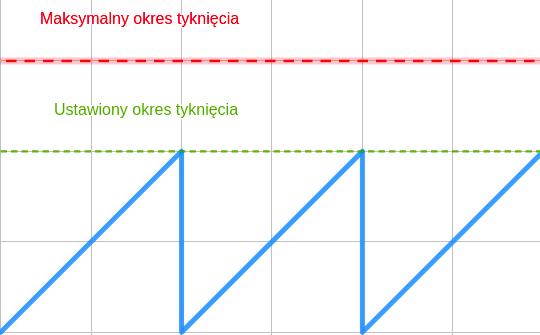
\includegraphics[scale=0.5]{images/pitcounter.png}
\caption{Zobrazowanie działania licznika PIT, a także przedstawienie ograniczeń związanych z ustawieniem wysokiej częstotliwości zegara - mniejszym okresem pomiędzy tyknięciami zegara}
\end{figure} 

Więc po upłynięciu okresu nasz licznik się resetuje, a w przypadku jeśli w którymś miejscu wyłączyliśmy przerwania to nie wiemy ile razy nasz licznik się przepełnił. Przerwania trzymane są w postaci maski bitowej (występuje / nie występuje) przez co jeśli nastąpiły dwa przepełnienia to potem tylko raz wywołujemy funkcję obsługującą przerwanie. Wcześniej dodawaliśmy tylko okres zegara w handlerze przerwania, ale powodowało to opóźnienia zegara. Teraz dodatkowo staramy się zauważyć przepełnienie w trakcie odczytu z zegara.

\begin{longlisting}
  \begin{minted}{c}
typedef struct pit_state {
  resource_t *regs;
  resource_t *irq_res;
  timer_t timer;
  bool noticed_overflow; /* noticed and handled the counter overflow */
  uint16_t period_cntr;  /* number of counter ticks in a period */
  /* values since last counter read */
  uint16_t prev_cntr16; /* number of counter ticks */
  /* values since initialization */
  uint32_t cntr_modulo; /* number of counter ticks modulo TIMER_FREQ*/
  uint64_t sec;         /* seconds */
} pit_state_t;

/* ... */
  
static bintime_t pit_timer_gettime(timer_t *tm) {
  device_t *dev = device_of(tm);
  pit_state_t *pit = dev->state;
  uint64_t sec;
  uint32_t ticks;
  WITH_INTR_DISABLED {
    pit_update_time(pit);
    sec = pit->sec;
    cntr_modulo = pit->cntr_modulo;
  }
  bintime_t bt = bintime_mul(tm->tm_min_period, ticks);
  bt.sec += sec;
  return bt;
}
  \end{minted}
  \caption{\href{https://mimiker.ii.uni.wroc.pl/source/xref/mimiker/sys/drv/pit.c?r=2609772a&mo=220&fi=9\#125}{Funkcja pit\_timer\_gettime} oraz \href{https://mimiker.ii.uni.wroc.pl/source/xref/mimiker/sys/drv/pit.c?r=2609772a&mo=220&fi=9\#9}{struktura pit\_state}}
  \label{lst:functimerpitgettime}
\end{longlisting}

Odczyt czasu z zegara następuje identycznie jak w przypadku zegara MIPSowego, gdzie odczytujemy liczbę sekund oraz tyknięć, których suma czasu nie tworzy pełnego okresu zegara, lecz wołana wcześniej funkcja \textbf{pit\_update\_time} różni się w zadaniach, które wykonuje.

\begin{longlisting}
  \begin{minted}{c}
static void pit_update_time(pit_state_t *pit) {
  assert(intr_disabled());
  @\llabel{pitupdateinit}@uint64_t last_sec = pit->sec;
  uint32_t last_cntr = pit->cntr_modulo;
  uint16_t now_cntr16 = pit_get_counter(pit);
  uint16_t ticks_passed = now_cntr16 - pit->prev_cntr16;
  @\llabel{pitoverflow}@if (pit->prev_cntr16 > now_cntr16) {
    pit->noticed_overflow = true;
    ticks_passed += pit->period_cntr;
  }

  /* We want to keep the last read counter value to detect possible future
   * overflows of our counter */
  pit->prev_cntr16 = now_cntr16;

  pit_incr_cntr(pit, ticks_passed);
  assert(last_sec < pit->sec ||
         (last_sec == pit->sec && last_cntr < pit->cntr_modulo));
  assert(pit->cntr_modulo < TIMER_FREQ);
}
  \end{minted}
  \caption{\href{https://mimiker.ii.uni.wroc.pl/source/xref/mimiker/sys/drv/pit.c?r=2609772a\#49}{Funkcja pit\_update\_time}}
  \label{lst:funcpitupdatetimer}
\end{longlisting}

Funkcja najpierw odczytuje poprzednie wartości zegara, następnie pobiera z zegara aktualny stan licznika i wylicza różnice pomiędzy ostatnią, a aktualnie odczytaną wartością \ref{pitupdateinit}. W przypadku kiedy aktualna liczba tyknięć jest mniejsza od poprzedniej \ref{pitoverflow} -- nastąpiło przepełnienie, a przerwanie nie zostało jeszcze obsłużone (ponieważ jeśli zostałoby obsłużone to wartość licznika zostałaby także zaktualizowana). Wtedy obsługujemy tą sytuacje oraz oznaczamy, że zauważyliśmy przepełnienie, aby handler nie powtórzył naszych obliczeń dla tego samego przepełnienia.

Następnie zapisujemy odczytane wartość licznika, inkrementujemy liczbę tyknięć zegara za pomocą \textbf{pit\_incr\_cntr} i za pomocą asercji sprawdzamy czy odmierzony czas przez nasz zegar 'nie cofa się', a także czy liczba tyknięć modulo jest mniejsza niż okres naszego zegara.

\begin{longlisting}
  \begin{minted}{c}
static inline void pit_incr_cntr(pit_state_t *pit, uint16_t ticks) {
  pit->cntr_modulo += ticks;
  if (pit->cntr_modulo >= TIMER_FREQ) {
    pit->cntr_modulo -= TIMER_FREQ;
    pit->sec++;
  }
}
  \end{minted}
  \caption{\href{https://mimiker.ii.uni.wroc.pl/source/xref/mimiker/sys/drv/pit.c?r=2609772a\#41}{Funkcja pit\_incr\_cntr}}
  \label{lst:funcpitincrticks}
\end{longlisting}


Funkcja ta aktualizuje liczbę tyknięć oraz dba, aby nie przekroczyły pełnego okresu zegara, który jest zliczany za pomocą liczby minionych sekund.

Warto zwrócić jeszcze uwagę na funkcję obsługującą przerwania tego zegara.

\begin{longlisting}
  \begin{minted}{c}
static intr_filter_t pit_intr(void *data) {
  pit_state_t *pit = data;

  @\llabel{pitcomment}@/* XXX: It's still possible for periods to be lost.
   * For example disabling interrupts for the whole period
   * without calling pit_gettime will lose period_cntr.
   * It is also possible that time suddenly jumps by period_cntr
   * due to the fact that pit_update_time() can't detect an overflow if
   * the current counter value is greater than the previous one, while
   * pit_intr() can thanks to the noticed_overflow flag. */
  @\llabel{pitupdate}@pit_update_time(pit);
  if (!pit->noticed_overflow)
    pit_incr_cntr(pit, pit->period_cntr);
  tm_trigger(&pit->timer);
  /* It is set here to let us know in the next interrupt if we already
   * considered the overflow */
  @\llabel{pitsetnoticed}@ppit->noticed_overflow = false;
  return IF_FILTERED;
}
  \end{minted}
  \caption{\href{https://mimiker.ii.uni.wroc.pl/source/xref/mimiker/sys/drv/pit.c?r=2609772a\#70}{Funkcja pit\_intr}}
  \label{lst:funcpitintr}
\end{longlisting}

Podobnie jak poprzednio najpierw aktualizujemy czas \ref{pitupdate} za pomocą funkcji \textbf{pit\_update\_time}, która może nie zauważyć przepełnienia licznika. Przykładowo minął pełen okres oraz jedno tyknięcie od poprzedniego odczytu. Wtedy stan licznika się zwiększył przez co nie możemy podejrzewać przepełnienia i dlatego jeśli nie zostało zauważone podczas aktualizacji odczytu handler dodaje ten okres. Pod koniec \ref{pitsetnoticed} oznaczamy \textbf{noticed\_overflow} jako fałsz, aby np. przy następnym przerwaniu wiedzieć, że przepełnienie nie zostało jeszcze obsłużone.

Odnośnie komentarza \ref{pitcomment} to takie podejście nie gwarantuje, że jeśli przerwania będą wyłączone na przynajmniej jeden okres to zaobserwujemy wszystkie przepełnienia.

\begin{figure}[ht]
\centering
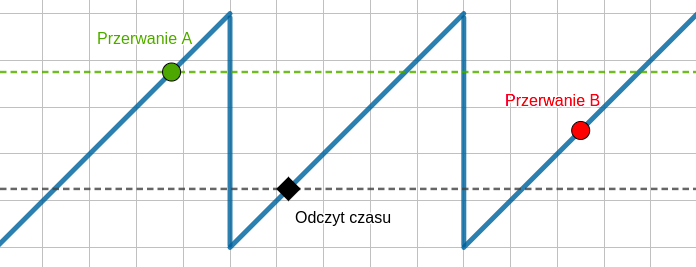
\includegraphics[scale=0.55]{images/pitinterrupt.png}
\caption{Przykład przedstawiający zgubienie tyknięcia zegara PIT}
\end{figure} 

Na powyższym przykładzie zakładając, że przerwania są wyłączone pomiędzy przerwaniem A i B (okres jest większy niż jedno tyknięcie, ale mniejszy niż dwa tyknięcia zegara). Mimo, że każda funkcja jest uruchamiana w innym tyknięciu to wciąż gubimy mierzenie jednego pełnego okresu, ponieważ odczyt czasu obsługuje pierwsze przepełnienie, ale przerwanie B nie jest "świadome", że nastąpiło przepełnienie pomiędzy jego obsługą, a ostatnim odczytem czasu.

W systemach *BSD korzysta się np. z bitu sprawdzającego czy przyszło przerwanie \cite{bib:pitbitpending}, aby zaktualizować czas. Innym stosowanym sposobem jest wykorzystanie MC146818 (RTC), który generuje przerwania ze stałą częstotliwością (zegar ten umożliwia generowanie przerwań ze znacznie wyższą częstotliwością niż pozwala odczytać czas), zaś zegar PIT ustawia się na najdłuższy możliwy okres taktowania, dzięki czemu można w pełni korzystać z 16 bitowego licznika, który oferuje \cite{bib:pitrtc}.


\section{Mierzenie czasu}
Przed podjęciem przeze mnie pracy, w jądrze systemu była dostępna jedynie prosta funkcja umożliwiająca dostęp do czasu ulotnego. Czyli czasu, który upłynął od momentu uruchomienia systemu sczytując wartość z zegara znajdującego się przy procesorze. Dodanie konwersji tm\_t do sekund, ustawienia czasu bootowania, a także implementacja gettimeofday umożliwiła śledzenie czasu w przestrzeni użytkownika.

\subsection{Wybór zegara}
Podczas inicjalizacji jądra należy wybrać zegar, który będzie służył do regularnego generowania przerwań, aby obsługiwać rutynę \textbf{clock\_cb} podobną do hardlocka i statclocka z FreeBSD.

\begin{longlisting}
  \begin{minted}{c}
static void clock_cb(timer_t *tm, void *arg) {
  bintime_t bin = binuptime();
  now = bt2st(&bin);
  stat_clock();
  callout_process(now);
  sched_clock();
}
  \end{minted}
  \caption{\href{https://mimiker.ii.uni.wroc.pl/source/xref/mimiker/sys/kern/clock.c?r=039f8f3e\#20}{Funkcja clock\_cb}}
  \label{lst:funcclockcb}
\end{longlisting}

Jej zadaniami jest aktualizowanie czasu systemowego (now), wywołanie funkcji stat\_clock odpowiedzialnej za zbieranie informacji o systemie, przetworzenie wszystkich calloutów, czyli zadań, których termin upłynął.
Rutyna po ich obsłużeniu wywołuje funkcję sched\_clock, która nalicza czas działania danego procesu.

Funkcją odpowiadającą za wybór zegara jest \textbf{init\_clock}, która wołana jest podczas uruchamiania systemu w funkcji \textbf{init\_main}, odpowiadającej za przygotowanie systemu do działania.

\begin{longlisting}
  \begin{minted}{c}
void init_clock(void) {
  @\llabel{tmreserve}@clock = tm_reserve(NULL, TMF_PERIODIC);
  if (clock == NULL)
    panic("Missing suitable timer for maintenance of system clock!");
  @\llabel{tminit}@tm_init(clock, clock_cb, NULL);
  @\llabel{tmstart}@if (tm_start(clock, TMF_PERIODIC | TMF_TIMESOURCE, (bintime_t){},
               HZ2BT(CLK_TCK)))
    panic("Failed to start system clock!");
  klog("System clock uses \'%s\' hardware timer.", clock->tm_name);
}
  \end{minted}
  \caption{\href{https://mimiker.ii.uni.wroc.pl/source/xref/mimiker/sys/kern/clock.c?r=039f8f3e\#28}{Funkcja init\_clock}}
  \label{lst:funcinitclock}
\end{longlisting}

Najpierw rezerwujemy zegar \ref{tmreserve} za pomocą, którego możemy wywoływać okresowo przerwania - \textbf{TMF\_PERIODIC}. Służy do tego funkcja \textbf{tm\_reserve}.

\begin{longlisting}
  \begin{minted}{c}
timer_t *tm_reserve(const char *name, unsigned flags) {
  timer_t *found = NULL;

  WITH_MTX_LOCK (&timers_mtx) {
    timer_t *tm;
    TAILQ_FOREACH (tm, &timers, tm_link) {
      if (is_reserved(tm))
        continue;
      if (name && strcmp(tm->tm_name, name))
        continue;
      if (!(tm->tm_flags & flags))
        continue;
      if (!found || found->tm_quality < tm->tm_quality)
        found = tm;
    }
    if (found)
      found->tm_flags |= TMF_RESERVED;
  }
  return found;
}
  \end{minted}
  \caption{\href{https://mimiker.ii.uni.wroc.pl/source/xref/mimiker/sys/kern/timer.c?r=3547949d\#75}{Funkcja tm\_reserve}}
  \label{lst:functmreserve}
\end{longlisting}

Funkcja ta najpierw za pomocą makra \textbf{WITH\_MTX\_LOCK} rezerwuje muteks \textbf{timers\_mtx} pozwalający na wyłączność korzystać z listy timerów, nastepnie korzystając z \textbf{TAILQ\_FOREACH} przechodzi po liście wszystkich zegarów, sprawdza czy nie są już zarezerwowane, a następnie jeśli chcieliśmy wybrać konkretny zegar o nazwie name to szuka pasującego wraz z flagami, które podaliśmy jako argument. Pod koniec jeśli udało się znaleźć zegar oznacza, że jest już zarezerwowany.

Następnie po rezerwacji zegara, inicjalizujemy \ref{tminit} go przy użyciu funkcji \textbf{tm\_init}.

\begin{longlisting}
  \begin{minted}{c}
int tm_init(timer_t *tm, tm_event_cb_t event, void *arg) {
  assert(is_reserved(tm));

  if (is_active(tm))
    return EBUSY;

  tm->tm_flags |= TMF_INITIALIZED;
  tm->tm_event_cb = event;
  tm->tm_arg = arg;
  return 0;
}
  \end{minted}
  \caption{\href{https://mimiker.ii.uni.wroc.pl/source/xref/mimiker/sys/kern/timer.c?r=3547949d\#119}{Funkcja tm\_init}}
  \label{lst:functminit}
\end{longlisting}

Funkcja ta sprawdza czy zegar nie jest już aktywny, a następnie uzupełnia pola odnośnie funkcji wołanej przez sygnał zegara, jej argumentu oraz flagi informującej o zainicjalizowaniu zegara.

Ostatnim etapem jest uruchomienie zegara \ref{tmstart} wraz z odpowiednimi flagami odnośnie trybu (\textbf{TMF\_PERIODIC}) i roli (\textbf{TMF\_TIMESOURCE} - źródło czasu) wraz z okresem wywoływań funkcji.

\begin{longlisting}
  \begin{minted}{c}
int tm_start(timer_t *tm, unsigned flags, const bintime_t start,
             const bintime_t period) {
  assert(is_initialized(tm));

  if (is_active(tm))
    return EBUSY;
  if (((tm->tm_flags & flags) & TMF_TYPEMASK) == 0)
    return ENODEV;
  if (flags & TMF_PERIODIC) {
    if (bintime_cmp(&period, &tm->tm_min_period, <) ||
        bintime_cmp(&period, &tm->tm_max_period, >))
      return EINVAL;
  }

  @\llabel{timerstart}@int retval = tm->tm_start(tm, flags, start, period);
  if (retval == 0)
    tm->tm_flags |= TMF_ACTIVE;
  if (flags & TMF_TIMESOURCE)
    time_source = tm;
  return retval;
}
  \end{minted}
  \caption{\href{https://mimiker.ii.uni.wroc.pl/source/xref/mimiker/sys/kern/timer.c?r=3547949d\#131}{Funkcja tm\_start}}
  \label{lst:functmstart}
\end{longlisting}

Głównym zadaniem tej funkcji jest sprawdzenie czy wszystkie argumenty są poprawne:
\begin{itemize}
    \item podany zegar jest zainicjalizowany
    \item zegar nie został jeszcze uruchomiony (wystartowany)
    \item podany okres tyknięcia jest w granicach operowania zegara
\end{itemize}

Następnie zegar jest startowany \ref{timerstart}, jeśli został poprawnie uruchomiony oznaczamy go jako aktywny. W przypadku kiedy zegar docelowo ma być naszym źródłem czasu przypisujemy, że ten zegar nim jest.


\subsection{Inicjalizacja czasu}
Podczas dodawania sterownika zegara RTC do systemu wykorzystuje się jego nieulotność. Podczas inicjalizacji systemu jądro wykrywa wszystkie podłączone urządzenia oraz jeśli jest to możliwe próbuje je się podłączyć do systemu za pomocą odpowiedniej funkcji (w tym przypadku \textbf{rtc\_attach}). Jednorazowo odczytujemy czas z zegara i uruchamiamy funkcję inicjalizującą czas uruchomienia systemu.

\begin{longlisting}
  \begin{minted}{c}
static int rtc_attach(device_t *dev) {
  /* ... */
  rtc_state_t *rtc = dev->state;
  /* ... */
  tm_t t;
  
  rtc_gettime(rtc->regs, &t);
  boottime_init(&t);

  return 0;
}
  \end{minted}
  \caption{\href{https://mimiker.ii.uni.wroc.pl/source/xref/mimiker/sys/drv/rtc.c?r=825ac182\#97}{Funkcja rtc\_attach}}
  \label{lst:funcrtcattach}
\end{longlisting}

\begin{longlisting}
  \begin{minted}{c}
static void boottime_init(tm_t *t) {
  time_t time = tm2sec(t);
  bintime_t bt = BINTIME(time);
  @\llabel{setclock}@tm_setclock(&bt);
}
  \end{minted}
  \caption{Inicjalizacja czasu bootowania za pomocą \href{https://mimiker.ii.uni.wroc.pl/source/xref/mimiker/sys/drv/rtc.c?r=825ac182\#38}{funkcji boottime\_init}}
  \label{lst:funcboottime}
\end{longlisting}

Czas jest konwertowany do reprezentacji bintime i uruchamiana jest funkcja, która ustawia czas \ref{setclock}.

\begin{longlisting}
  \begin{minted}{c}
time_t tm2sec(tm_t *t) {
  if (t->tm_year < 70)
    return 0;

  const int32_t year_scale_s = 31536000, day_scale_s = 86400,
                hour_scale_s = 3600, min_scale_s = 60;
  time_t res = 0;
  static const int month_in_days[12] = {0,   31,  59,  90,  120, 151,
                                        181, 212, 243, 273, 304, 334};

  res += (time_t)month_in_days[t->tm_mon] * day_scale_s;
  /* Extra days from leap years which already past (EPOCH) */
  res += (time_t)((t->tm_year + 1900) / 4 - (1970) / 4) * day_scale_s;
  res -= (time_t)((t->tm_year + 1900) / 100 - (1970) / 100) * day_scale_s;
  res += (time_t)((t->tm_year + 1900) / 400 - (1970) / 400) * day_scale_s;

  /* If actual year is a leap year and the leap day passed */
  if (t->tm_mon > 1 && (t->tm_year % 4) == 0 &&
      ((t->tm_year % 100) != 0 || (t->tm_year + 1900) % 400) == 0)
    res += day_scale_s;

  /* (t.tm_mday - 1) - cause days are in range [1-31] */
  return (time_t)(t->tm_year - 70) * year_scale_s +
         (t->tm_mday - 1) * day_scale_s + t->tm_hour * hour_scale_s +
         t->tm_min * min_scale_s + t->tm_sec + res;
}
  \end{minted}
  \caption{Konwersja z tm\_t do sekund za pomocą \href{https://mimiker.ii.uni.wroc.pl/source/xref/mimiker/sys/kern/time.c?r=9505a819\#124}{funkcji tm2sec}}
  \label{lst:functm2sec}
\end{longlisting}

Reprezentacją czasu w formie kalendarzowej oprócz już wcześniej wspomnianych problemów z nieefektywnością porównań, problemy pojawiają się również pod względem  konwersji tej struktury do sekund. W funkcji \textbf{tm2sec} korzystając ze stałych reprezentujących ile sekund zawiera rok nieprzestępny, dzień itd. umożliwia nam proste przekonwertowanie tych formatów do sekund. Potrzebne są też nam dni, w poszczególnych miesiącach, gdzie korzystamy z tablicy \textbf{month\_in\_days}, która przechowuje informacje ile dni upłynęło przed danym miesiącem. Następnie należy obliczyć dni przestępne, które nie zostały wcześniej uwzględnione.

\begin{longlisting}
  \begin{minted}{c}
void tm_setclock(const bintime_t *bt) {
    bintime_t bt1 = *bt, bt2;
    /* TODO: Add (spin) lock for settime */
    bt2 = binuptime();
    /* Setting boottime - this is why we subtract time elapsed since boottime */
    bintime_sub(&bt1, &bt2);
    boottime = bt1;
  }
  \end{minted}
  \caption{\href{https://mimiker.ii.uni.wroc.pl/source/xref/mimiker/sys/kern/timer.c?r=3547949d\#110}{Funkcja tm\_setclock}}
  \label{lst:functmsetclock}
\end{longlisting}

Podczas ustawiania czasu odejmujemy wartość odczytaną od pożądanej daty, ponieważ ustawiamy czas uruchomienia systemu, a nie aktualnego momentu.

\subsection{Dostęp do czasu w przestrzeni użytkownika}
Ustawianie czasu uruchomienia (bootowania) pozwoliło na odczyt czasu rzeczywistego w postaci UTC. Wywołaniem systemowym za pomocą którego można pozyskać tą wartość w przestrzeni użytkownika jest \textbf{gettimeofday} \cite{bib:gettime-manual}.
\begin{longlisting}
  \begin{minted}{c}
int gettimeofday(timeval_t *tp, void *tzp) {
  if (tp) {
    timespec_t ts;
    clock_gettime(CLOCK_REALTIME, &ts);
    tp->tv_sec = ts.tv_sec;
    tp->tv_usec = ts.tv_nsec / 1000;
  }
  return 0;
}
  \end{minted}
  \caption{\href{https://mimiker.ii.uni.wroc.pl/source/xref/mimiker/lib/libc/sys/gettimeofday.c?r=2a3a339e\#3}{Funkcja gettimeofday}}
  \label{lst:funcgettimeofday}
\end{longlisting}

Wskaźnik \textbf{tzp} historycznie był wykorzystywany do odczytu strefy czasowej (ang. time zone pointer), lecz nie ma prostego algorytmu, który umożliwiłby określenie strefy czasowej, a dodatkowo może to ulegać zmianie poprzez polityczne decyzje, dlatego porzucono ideę obsługiwania stref czasowych w taki sposób \cite{bib:gettime-manual}.

Funkcja wołana z poziomu jądra obsługująca wywołanie \textbf{clock\_gettime} \cite{bib:clock_gettime} jest \textbf{do\_clock\_gettime}.

\begin{longlisting}
  \begin{minted}{c}
int do_clock_gettime(clockid_t clk, timespec_t *tp) {
  bintime_t bin;
  switch (clk) {
    case CLOCK_REALTIME:
      bin = bintime();
      break;
    case CLOCK_MONOTONIC:
      bin = binuptime();
      break;
    default:
      return EINVAL;
  }
  bt2ts(&bin, tp);
  return 0;
}
  \end{minted}
  \caption{\href{https://mimiker.ii.uni.wroc.pl/source/xref/mimiker/sys/kern/time.c?r=9505a819\#11}{Funkcja do\_clock\_gettime}}
  \label{lst:funcdoclockgettime}
\end{longlisting}

Opcja \textbf{CLOCK\_REALTIME} służy do odczytu czasu EPOCH, zaś za pomocą \textbf{CLOCK\_MONOTONIC} odczytujemy czasu, który upłynął od uruchomienia systemu.

\begin{longlisting}
  \begin{minted}{c}
bintime_t bintime(void) {
  bintime_t retval = binuptime();
  @\llabel{bootadd}@bintime_add(&retval, &boottime);
  return retval;
}
  \end{minted}
  \caption{\href{https://mimiker.ii.uni.wroc.pl/source/xref/mimiker/sys/kern/timer.c?r=3547949d\#184}{Funkcja bintime}}
  \label{lst:funcbintime}
\end{longlisting}

Funkcja \textbf{bintime} do czasu, który upłynął od bootowania dodaje dodatkowo czas, w którym system został uruchomiony \ref{bootadd}.

\begin{longlisting}
  \begin{minted}{c}
bintime_t binuptime(void) {
  /* XXX: probably a race condition here */
  timer_t *tm = time_source;
  if (tm == NULL)
    return BINTIME(0);
  return tm->tm_gettime(tm);
}
  \end{minted}
  \caption{\href{https://mimiker.ii.uni.wroc.pl/source/xref/mimiker/sys/kern/timer.c?r=3547949d\#176}{Funkcja binuptime}}
  \label{lst:funcbinuptime}
\end{longlisting}

Funkcja \textbf{binuptime} sczytuje bezpośrednio czas, który został naliczony przez zegar od rozpoczęcia jego działania. 

Implementacja gettimeofday umożliwiła wołanie komendy \textbf{date} z terminala systemu, co pozwala na śledzenie czasu w przestrzeni użytkownika.


\begin{figure}[ht]
\centering
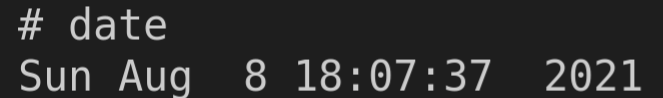
\includegraphics[scale=0.55]{date.png}
\caption{Przykładowe wywołanie komendy date w systemie Mimiker.}
\end{figure}


\section{Scheduler}


Scheduler ten jest dużo prostszy niż ULE i polega na przydzieleniu kwantu czasu wątkowi, a następnie jego odliczaniu.

\begin{longlisting}
  \begin{minted}{c}
void sched_clock(void) {
  assert(intr_disabled());

  thread_t *td = thread_self();

  if (td != PCPU_GET(idle_thread)) {
    WITH_SPIN_LOCK (td->td_lock) {
      @\llabel{kwant}@if (--td->td_slice <= 0)
        td->td_flags |= TDF_NEEDSWITCH | TDF_SLICEEND;
    }
  }
}
  \end{minted}
  \caption{\href{https://mimiker.ii.uni.wroc.pl/source/xref/mimiker/sys/kern/sched.c?r=c1104992\#174}{Funkcja sched\_clock}}
  \label{lst:funcschedclock}
\end{longlisting}

Podobnie jak scheduler ULE w Mimikerze również korzystamy z danych zebranych podczas rutyny --- clock\_cb, a dokładniej \textbf{sched\_clock}. W przypadku kiedy proces nie jest procesem jałowym (ang. idle) i wykorzystał swój czas \ref{kwant} to wątek oznacza się, że należy wykonać zmianę kontekstu (\textbf{TDF\_NEEDSWITCH}) oraz przydzielony kwant czasu został wykorzystany (\textbf{TDF\_SLICEEND}).

\section{Sen}

W systemach operacyjnych zadania mogą oczekiwać na wydarzenia na trzy sposoby \cite{bib:locking-manual}:
\begin{itemize}
    \item \textbf{Sen ograniczony} (ang. bounded sleep) zwany też "blokującym" występuje, gdy wątek pozostaje uśpiony dopóki nie zostanie zwolniona blokada (występuje np. w trakcie oczekiwania na muteks)
    \item \textbf{Sen nieograniczony} (ang. unbounded sleep) występuje, gdy wątek czeka na zewnętrzne zdarzenie (np. wywołanie systemowe sleep \cite{bib:sleep-manual})
    \item \textbf{Aktywne czekanie} (ang. busy waiting) oznacza czekanie np. w pętli while dopóki nie zostanie spełniony warunek lub zwolniony zasób (np. blokada spinlock)
\end{itemize}

\subsection{Usypianie o wysokiej rozdzielczości}

Wywołanie systemowe \textbf{nanosleep} \cite{bib:nanosleep-manual}, które zostało przeze mnie dodane, służy do wprowadzenia wątku w sen nieograniczony o wysokiej rozdzielczości (dokładność do nanosekund) w przestrzeni użytkownika naszego systemu.

\begin{longlisting}
  \begin{minted}{c}
int nanosleep(const timespec_t *rqtp, timespec_t *rmtp) {
  return clock_nanosleep(CLOCK_REALTIME, 0, rqtp, rmtp);
}
  \end{minted}
  \caption{\href{https://mimiker.ii.uni.wroc.pl/source/xref/mimiker/lib/libc/sys/nanosleep.c?r=bea91cda\#3}{Funkcja nanosleep}}
  \label{lst:funcnanosleep}
\end{longlisting}

Wywołanie systemowe, może się nie udać kiedy argumenty są nieprawidłowe (np. ujemne sekundy), nastąpił błąd podczas kopiowania pamięci z przestrzeni użytkownika do jądra lub sygnał został dostarczony do wątku, który spał. Wtedy pozostały czas snu, zostaje umieszczony w strukturze wskazywanej przez rmtp (jeśli została podana).

Funkcja przyjmuje dwa parametry - \textbf{rqtp} wskaźnik na strukturę zawierającą informacje ile zadanie chce spać (ang. requested time pointer) oraz \textbf{rmtp}, który wskazuje na strukturę zwracającą pozostały czas snu (ang. remaining time pointer), który nie został odczekany, np przerwany przez sygnał. 

Wołana jest funkcja \textbf{clock\_nanosleep} \cite{bib:clock_nanosleep}, która z poziomu jądra jest obsługiwana przez \textbf{do\_clock\_nanosleep}. Dodatkowo przyjmuje ona argumenty związane z rodzajem zegara jakim jest dokonywany sen (podobnie jak w do\_clock\_gettime), zaś flaga umożliwia ustawienie \textbf{TIMER\_ABSTIME}, wtedy \textbf{rqtp} jest wykorzystywany jako punkt w czasie, do którego chcemy spać, w przeciwnym przypadku śpimy tyle czasu ile czasu ile podano.

\begin{longlisting}
  \begin{minted}{c}
int do_clock_nanosleep(clockid_t clk, int flags, timespec_t *rqtp,
                       timespec_t *rmtp) {
  /* rmt - remaining time, rqt - requested time, p - pointer */
  timespec_t rmt_start, rmt_end, rmt;
  systime_t timo;
  int error, error2;

  @\llabel{ts2timo}@if ((error = ts2timo(clk, flags, rqtp, &timo, &rmt_start))) {
    if (error == ETIMEDOUT)
      goto timedout;
    return error;
  }

  do {
    @\llabel{sleepq}@error = sleepq_wait_timed((void *)(&rmt_start), __caller(0), timo);
    if (error == ETIMEDOUT)
      goto timedout;

    if ((error2 = do_clock_gettime(clk, &rmt_end)))
      return error2;

    @\llabel{do_clock_nanosleepcheckflag}@if (flags == TIMER_ABSTIME) {
      timespecsub(rqtp, &rmt_end, &rmt);
    } else {
      timespecsub(&rmt_end, &rmt_start, &rmt);
      timespecsub(rqtp, &rmt, &rmt);
    }
    if (rmt.tv_sec < 0)
      timespecclear(&rmt);

    @\llabel{nanosleeprmtp}@if (rmtp)
      *rmtp = rmt;
    if (error)
      return error;

    timo = ts2hz(&rmt);
  } while (timo > 0);

  return 0;

 @\llabel{timedout}@etimedout:
  if (rmtp)
    rmtp->tv_sec = rmtp->tv_nsec = 0;
  return 0;
}
  \end{minted}
  \caption{\href{https://mimiker.ii.uni.wroc.pl/source/xref/mimiker/sys/kern/time.c?r=9505a819\#78}{Funkcja do\_clock\_nanosleep}}
  \label{lst:funcfoclocknanosleep}
\end{longlisting}

Najpierw za pomocą funkcji \textbf{ts2timo} (timo - skrót od time out) obliczamy ile tyknięć systemowych potrzeba, aby termin się przedawnił \ref{ts2timo}. Następnie za pomocą kolejki uśpionych wątków \ref{sleepq} wprowadza się wątek w sen nieograniczony (więcej można znaleźć pod \cite{bib:jpszcz}), gdzie próbujemy odczekać ten okres. Jeśli funkcja zwróci \textbf{ETIMEDOUT} oznacza to, że termin minął i możemy wyczyścić rmtp gdy istnieje taka potrzeba i wyjść \ref{timedout}. Jeśli jednak nie minął termin to chcemy odczytać aktualny czas i w zależności jaka flaga jest ustawiona to obliczyć ile czasu pozostało do końca terminu \ref{do_clock_nanosleepcheckflag}. Może się okazać, że w trakcie przetwarzania termin minął, wtedy czyścimy rmt. Jeśli rmtp było ustawione to zapisujemy w nim wartość \ref{nanosleeprmtp}. Jeśli nastąpił błąd to wychodzimy z procedury, a w przeciwnym przypadku kontynuujemy sen jeśli termin nie upłynął lub kończymy działanie.

\begin{longlisting}
  \begin{minted}{c}
static int ts2timo(clockid_t clock_id, int flags, timespec_t *ts,
                   systime_t *timo, timespec_t *start) {
  int error;
  *timo = 0;

  @\llabel{ts2timocheck}@if (timespec_invalid(ts) || (flags & ~TIMER_ABSTIME))
    return EINVAL;

  if ((error = do_clock_gettime(clock_id, start)))
    return error;

  if (flags & TIMER_ABSTIME)
    timespecsub(ts, start, ts);

  @\llabel{ts2timoexp}@if ((ts->tv_sec == 0 && ts->tv_nsec == 0) || ts->tv_sec < 0)
    return ETIMEDOUT;

  *timo = ts2hz(ts);

  return 0;
}
  \end{minted}
  \caption{\href{https://mimiker.ii.uni.wroc.pl/source/xref/mimiker/sys/kern/time.c?r=9505a819\#56}{Funkcja ts2timo}}
  \label{lst:functs2timo}
\end{longlisting}

Funkcja \textbf{ts2timo} służy do obliczenia ile tyknięć systemowych zostało do końca terminu wraz z uwzględnieniem opcji czy termin oznacza do kiedy chcemy skończyć (flaga TIMER\_ABSTIME) czy jak długo chcemy czekać (brak flagi). Najpierw sprawdzamy poprawność wejścia \ref{ts2timocheck} --- poprawność struktury ts oraz czy nie ustawiono flag, które nie są wspierane przez funkcję. Następnie odczytujemy czas i jeśli ustawiliśmy flagę TIMER\_ABSTIME to odejmujemy od terminu aktualny czas, co pozwala nam obliczyć ile czasu chcemy czekać, następnie sprawdzamy czy termin już nie upłynął \ref{ts2timoexp}, jeśli nie to konwertujemy czas do liczby tyknięć systemu za pomocą \textbf{ts2hz}.

Implementacja ta dostarczyła nam opcję snu o wysokiej rozdzielczości w przestrzeni użytkownika, a także działanie funkcji \textbf{sleep} \cite{bib:sleep-manual} z biblioteki standardowej C, która korzysta w swej implementacji z nanosleepa.


\chapter{Profilowanie}
Profilowanie służy do zbierania danych umożliwiających analizowanie oprogramowania pod względem wydajnościowym. Samo analizowanie danych jest skomplikowanym procesem i wymaga zwrócenia uwagi na wiele aspektów (m.in. stabilność systemu, jakie wywołania są śledzone). Dlatego głównie skupimy się na tym w jaki sposób pozyskuje się dane, co nam one umożliwiają, a także przedstawię przykładowe narzędzia i ich funkcjonowanie.

\section{Sposoby zbierania informacji} 
Dane zbierane podczas profilowania różnią się sposobem ich pozyskania. Przybliżę najważniejsze z nich, a o innych można przeczytać w \cite{bib:denis}.

\subsection{Instrumentacja}

Metoda ta polega na umieszczeniu dodatkowego kodu w programie do zbierania informacji podczas działania oprogramowania. Najprostszą formą instrumentacji jest używanie komunikatów diagnostycznych (np. za pomocą printf). Podejście to pozwala głównie na informowaniu, który fragment kodu jest wywoływany, a nie np. jak długo, przez co sposób ten jest często łączony z innymi metodami, aby dać lepszy obraz działania systemu. Sama instrumentacja wydłuża czas wykonania się programu, ponieważ kod instrumentacji też musi zostać wykonany. Dlatego ważne, aby była efektywna i nie wpływała w znaczący sposób na oprogramowanie. Wykorzystywana jest np. do zliczania wywołań funkcji.

\subsection{Śledzenie}

Wykorzystuje się w podobnych celach co instrumentację, ale śledzenie opiera się na już istniejącej instrumentacji lub infrastrukturze. Najbardziej znanym przykładem jest polecenie strace z Linuxa, które pozwala śledzić wywołania systemowe (ang. system call). Złożoność obliczeniowa śledzenia zależy głównie od samego programu, np. strace na programie, który nie dokonuje dużej liczby wywołań systemowych nie wnosi dużego obciążenia w porównaniu do programu, który dokonuje ich dużo więcej. Może być wykorzystywany np. do badania interakcji między programem, a jądrem.

\subsection{Próbkowanie}

Najbardziej rozpowszechniona metoda polega na sprawdzeniu co pewien okres jaka funkcja jest wykonywana. Sposób ten często pozwala na stworzenie np. 'mapy ciepła' (ang. heat map) funkcji względem konsumpcji procesora. Każde trafienie w adres kodu należącego do funkcji podczas próbkowania możemy traktować jako korzystanie z procesora podczas tego okresu. Taka metoda przy założeniu, że żadna funkcja nie zsynchronizuje się z próbkowaniem pozwala dobrze odzwierciedlić czas działania poszczególnych funkcji. Założenie to nie zawsze jest spełnione, mimo tego próbkowanie dostarcza wystarczająco wiarygodnych informacji.

\section{Narzędzia do profilowania}

\subsection{gprof}

Narzędzie UNIXowe, będące następnikiem \textbf{prof}. Pozwala zbudować graf wywołań, zlicza ile razy każda funkcja została wywołana oraz szacuje czas ich działania \cite{bib:gprof}. W swojej implementacji bazuje na instrumentacji, która pozwala na wyliczenie dwóch pierwszych własności, a dodatkowo próbkowanie pozwala estymować korzystanie z procesora przez funkcje. 

\subsection{perf}

Najbardziej powszechnie stosowane narzędzie do analizy wydajności jądra Linuxa \cite{bib:perf}. Jest bardzo rozbudowane i wykorzystuje (o ile to możliwe) liczniki sprzętowe (np. licznik wykonanych instrukcji \cite{bib:perf}), tracepointy czy próbkowanie. Tracepointy są to zazwyczaj już zinstrumentowane fragmenty kodu, są umieszczone np. przy operacjach na systemie plików lub wydarzeniach TCP/IP, istnieje także możliwość ich dynamicznego tworzenia \cite{bib:perf}. Pomijając szacowanie ile czasu funkcje były wykonywane, narzędzie to jest dużo bardziej rozbudowane i pozwala na zliczanie nietrafionych odwołań do pamięci cache (ang. cache miss) czy źle przewidzianych rozgałęzień kodu (ang. branch misprediction).


\subsection{VTune}

Międzyplatformowe narzędzie firmy Intel służące do optymalizacji \cite{bib:vtune}. Wspiera wielowątkowość, śledzenie konsumpcji pamięci czy też zachowania wyjścia i wejścia. Ciekawą funkcjonalnością jest możliwość prezentacji jak długo dany fragment kodu był wykonywany, co pozwala na wykrywanie wąskich gardeł w naszym kodzie.

\section{Profiler gprof}

\textbf{Gprof} pozwala na profilowanie programów w językach, które wspiera np. kompilator gcc. W pierwszej kolejności podczas kompilacji programu należy ustawić flagi \textbf{-pg}, które odpowiadają za gprofa i przygotowują program do zbierania danych. Następnie po zakończeniu działania programu pojawi się plik wyjściowy \textbf{gmon.out}, który należy przetworzyć za pomocą komendy \textbf{gprof}, np. wpisując "gprof obraz\_programu gmon.out". Narzędzie przetworzy dane zebrane w gmon.out i połączy je z symbolami zawartymi w obrazie programu.

Gprof pozwala zaprezentować dane w trzech postaciach:
\begin{itemize}
    \item płaskiego profilowania (ang. flat profile) - przedstawia ile czasu program spędził w każdej funkcji i ile razy każda z tych funkcji była wołana
    \item grafu wywołań (ang. call graph) - prezentuje dla każdej funkcji jakie funkcje wołała i ile razy
    \item listowania źródeł z adnotacjami (ang. annotated source longlisting) - jest kopią kodu źródłowego wraz z etykietą ile razy wołana była dana linia programu
\end{itemize}

Na podstawie \cite{bib:gprof-out} omówię każdą z postaci:

\subsection{Płaskie profilowanie}
\begin{longlisting}
  \begin{minted}{c}
Flat profile:

Each sample counts as 0.01 seconds.
  %   cumulative   self              self     total           
 time   seconds   seconds    calls  ms/call  ms/call  name    
 33.34      0.02     0.02     7208     0.00     0.00  open
 16.67      0.03     0.01      244     0.04     0.12  offtime
 16.67      0.04     0.01        8     1.25     1.25  memccpy
 16.67      0.05     0.01        7     1.43     1.43  write
 16.67      0.06     0.01                             mcount
  0.00      0.06     0.00      236     0.00     0.00  tzset
  0.00      0.06     0.00      192     0.00     0.00  tolower
  0.00      0.06     0.00       47     0.00     0.00  strlen
  0.00      0.06     0.00       45     0.00     0.00  strchr
  0.00      0.06     0.00        1     0.00    50.00  main
  0.00      0.06     0.00        1     0.00     0.00  memcpy
  0.00      0.06     0.00        1     0.00    10.11  print
  0.00      0.06     0.00        1     0.00     0.00  profil
  0.00      0.06     0.00        1     0.00    50.00  report
...
  \end{minted}
  \caption{Przykładowy wynik płaskiego profilowanie funkcji}
  \label{lst:flatprof}
\end{longlisting}

Na górze dostajemy informację co jaki okres próbkowany jest program. każda linia zawiera funkcje, które są posortowane malejąco względem czasu wykonania.

Informacje zawarte w kolumnach:
\begin{itemize}
    \item \% time - ile procent czasu całkowitego funkcja się wykonywała, inaczej ile procent próbkowań trafiło na tą funkcję
    \item cumulative seconds - sumaryczna liczba sekund poświęconych na wykonanie tej funkcji wraz z wylistowanymi funkcjami nad nią
    \item self seconds - ile czasu sumarycznie wykonywały się wszystkie wywołania funkcji
    \item calls - liczba wywołań funkcji (jeśli funkcja nie jest instrumentowana pole pozostaje puste)
    \item self ms/call - średnia liczba milisekund spędzonych podczas jednego wywołania funkcji (jeśli funkcja nie jest profilowana pole pozostaje puste)
    \item total ms/call - średnia liczba milisekund spędzonych w funkcji oraz w funkcjach, które woła
    \item name - nazwa funkcji
\end{itemize}

\subsection{Graf wywołań}

Informuje nas ile czasu spędzono w każdej funkcji oraz w jej dzieciach (funkcjach wołanych przez nią).
\begin{longlisting}
  \begin{minted}{c}
granularity: each sample hit covers 2 byte(s) for 20.00% of 0.05 seconds

index % time    self  children    called     name
                                                 <spontaneous>
[1]    100.0    0.00    0.05                 start [1]
                0.00    0.05       1/1           main [2]
                0.00    0.00       1/2           on_exit [28]
                0.00    0.00       1/1           exit [59]
-----------------------------------------------
                0.00    0.05       1/1           start [1]
[2]    100.0    0.00    0.05       1         main [2]
                0.00    0.05       1/1           report [3]
-----------------------------------------------
                0.00    0.05       1/1           main [2]
[3]    100.0    0.00    0.05       1         report [3]
                0.00    0.03       8/8           timelocal [6]
                0.00    0.01       1/1           print [9]
                0.00    0.01       9/9           fgets [12]
                0.00    0.00      12/34          strncmp <cycle 1> [40]
                0.00    0.00       8/8           lookup [20]
                0.00    0.00       1/1           fopen [21]
                0.00    0.00       8/8           chewtime [24]
                0.00    0.00       8/16          skipspace [44]
-----------------------------------------------
[4]     59.8    0.01        0.02       8+472     <cycle 2 as a whole>	[4]
                0.01        0.02     244+260         offtime <cycle 2> [7]
                0.00        0.00     236+1           tzset <cycle 2> [26]
-----------------------------------------------
  \end{minted}
  \caption{Przykładowy graf wywołań}
  \label{lst:graphcallprof}
\end{longlisting}

Każdy wpis na temat funkcji i jej dzieci jest oddzielony przerywaną linią.

Linijka z zaznaczonym indeksem odnosi się do funkcji, która jest opisywana, wpisy nad nią opisują funkcję, które ją wołały, a pod nią, które są przez nią wołane. Wpisy są posortowane po czasie spędzonym w funkcji i jej dzieciach.

Opiszę znaczenie kolumn z podziałem na rodzaj wpisu: funkcja wołająca (1), funkcja główna (2), funkcja wołana (3). 

\begin{itemize}
    \item index - 
    \begin{enumerate}
        \item puste
        \item unikalny indeks funkcji
        \item puste
    \end{enumerate}
    
    \item \% time - 
    \begin{enumerate}
        \item puste
        \item procent czasu spędzonego w tej funkcji biorąc pod uwagę sumaryczny czas spędzony w funkcji oraz w funkcjach wołanych
        \item puste
    \end{enumerate}
    \item self -
    \begin{enumerate}
        \item szacowany czas spędzony tylko w funkcji głównej wołanej przez tą funkcję
        \item liczba sekund spędzonych w funkcji 
        \item szacowana liczba sekund spędzonych tylko w funkcji, gdy była zawołana przez funkcję główną
    \end{enumerate}
    \item children -
    \begin{enumerate}
        \item szacowany czas spędzony w dzieciach przez funkcję główna, gdy była wołana przez tą funkcję
        \item czas spędzony w funkcjach wołanych przez funkcje główną
        \item szacowana liczba sekund spędzona w dzieciach, jeśli ta funkcja była wołana przez funkcję główną
    \end{enumerate}
    \item called - 
    \begin{enumerate}
        \item liczba wywołań funkcji głównej przez tą funkcję podzielona przez totalną sumę wywołań funkcji głównej z pominięciem wywołań rekurencyjnych
        \item sumaryczna liczba wywołań funkcji głównej, jeśli funkcja była wykonywana rekurencyjnie wtedy osobno po + pojawia się liczba wywołań rekurencyjnych
        \item pierwsza liczba reprezentuje liczbę wywołań tej funkcji przez funkcję główna, a liczba po znaku / oznacza sumaryczną liczbę wywołań tej funkcji z pominięciem wywołań rekurencyjnych
    \end{enumerate}
    
    \item name - nazwy funkcji oraz jej indeks
\end{itemize}

\subsection{Listowanie źródeł}

Jest jeszcze trzecia opcja prezentacji informacji, ale wymaga ona dodatkowego skompilowania programu z flagą -a (nie wspieramy tego w Mimikerze).

\begin{longlisting}
  \begin{minted}{c}
                ulg updcrc(s, n)
                    uch *s;
                    unsigned n;
            2 ->{
                    register ulg c;
                
                    static ulg crc = (ulg)0xffffffffL;
                
            2 ->    if (s == NULL) {
            1 ->	c = 0xffffffffL;
            1 ->    } else {
            1 ->	c = crc;
            1 ->        if (n) do {
        26312 ->            c = crc_32_tab[...];
26312,1,26311 ->        } while (--n);
                    }
            2 ->    crc = c;
            2 ->    return c ^ 0xffffffffL;
            2 ->}
  \end{minted}
  \caption{Przykładowe listowanie źródeł}
  \label{lst:srclist}
\end{longlisting}

Metoda ta informuje ile razy linia kodu funkcji została wykonana, np. instrukcja \textbf{c = crc\_32\_tab[...];} została wykonana 26312 razy. W przypadku while'a stosuje się notację 26312,1,26311, które oznacza sumaryczne wykonania, jedno wyjście z pętli, a 26311 razy skoczyło ponownie na początek pętli.

\chapter{Profilowanie jądra w Mimikerze}

Narzędzie, które zaimplementowałem nazywa się kgprof (kernel gprof). Jest ono oparte na uniwersalnym narzędziu gprof \cite{bib:gprof} służy do profilowania jądra i przestrzeni użytkownika, a nasz profile działa tylko w jądrze. Narzędzie to było najbardziej uniwersalne względem różnych platform/architektur, a także udostępnia narzędzie do analizowania zebranych danych. 


\section{Implementacja kgprofa}
Jak już było to wyżej wspomniane, narzędzie to umożliwia budowanie grafu wywołań funkcji wraz z liczbą tych wywołań, a także estymowanie ile czasu działała taka funkcja. Aby móc zbierać wszystkie te informacje potrzebne są odpowiednie struktury danych, w których je zbierzemy.

\subsection{Kluczowe struktury}

\textbf{Tostruct\_t} to struktura, która umożliwia budowanie grafu i jest reprezentacją krawędzi skierowanej, w której trzymamy informacje o wołanej funkcji (ang. calle).

\begin{longlisting}
  \begin{minted}{c}
typedef struct tostruct {
  u_long selfpc;
  long count;
  u_short link;
} tostruct_t;
  \end{minted}
  \caption{\href{https://mimiker.ii.uni.wroc.pl/source/xref/mimiker/include/sys/gmon.h?r=27b8c19a\#102}{Struktura tostruct\_t}}
  \label{lst:structtostruct}
\end{longlisting}

 Wykorzystuje się ją do reprezentacji węzła (ang. node) listy jednokierunkowej wołanych funkcji.
 
\begin{itemize}
    \item \textbf{selfpc} adres wołanej funkcji
    \item \textbf{count} liczba wywołań tej funkcji przez właściciela
    \item \textbf{link} następny element listy (0 - koniec listy)
\end{itemize}

Po skompilowaniu pamięć jądra jest podzielona na segmenty:

\begin{figure}[ht]
\centering
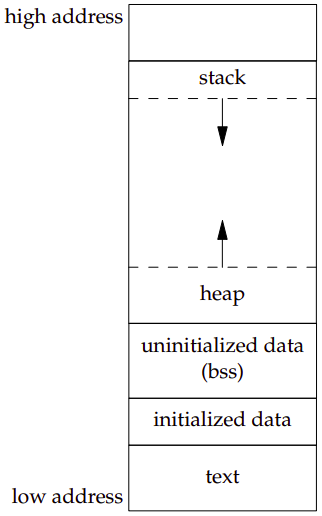
\includegraphics[scale=0.4]{images/memory.png}
\caption{Wizualizacja przestrzeni adresowej programu \cite{bib:apue}}
\end{figure} 

Sekcja text, która po skompilowaniu ma określony rozmiar i jest zazwyczaj dostępna tylko do odczytu (ang. read-only). Przechowuje ona instrukcje maszynowe programu, które wykonuje CPU \cite{bib:apue}. Właśnie na adres z tej przestrzeni adresowej wskazuję selfpc.

Link jest wartością, a nie wskaźnikiem jak to zazwyczaj bywa, dlatego że podczas inicjalizacji profilera alokuje się tablicę tos (opiszę ją poniżej). Tablica alokowana jest ze ściśle określonym rozmiarem (zależnym od rozmiaru sekcji text). Komórki tej tablicy reprezentują węzły różnych list. Więc zamiast wskaźnika na następny węzeł mamy indeks komórki, w której znajduje się kolejny węzeł (lub 0 w przypadku ostatniego węzła).

Podejście to pozwala na zminimalizowanie kosztu zbierania danych w trakcie działania programu, przez ominięcie dynamicznej alokacji pamięci. Drugim powodem jest fakt, że alokator pamięci zakłada, że przerwania są włączone, a podczas wykonywania kodu instrumentacji nie jesteśmy w stanie zapewnić czy instrumentowane funkcje ich nie wyłączyły.

Następna struktura umożliwia dostęp do wszystkich informacji zebranych przez profiler - \textbf{gmonparam\_t}:

\begin{longlisting}
  \begin{minted}{c}
typedef unsigned short HISTCOUNTER;
  /* ... */
typedef struct gmonparam {
  int state;
  HISTCOUNTER *kcount;
  u_long kcountsize;
  u_short *froms;
  u_long fromssize;
  struct tostruct *tos;
  u_long tossize;
  long tolimit;
  u_long lowpc;
  u_long highpc;
  u_long textsize;
  u_long hashfraction;
} gmonparam_t;
  \end{minted}
  \caption{\href{https://mimiker.ii.uni.wroc.pl/source/xref/mimiker/include/sys/gmon.h?r=27b8c19a\#111}{Struktura gmonparam\_t}}
  \label{lst:structgmonparam}
\end{longlisting}

Struktura ta zawiera całość zebranych informacji o badanym systemie oraz dodatkowo przechowuje metadane związane z profilowaniem. Używane poniżej pojęcie \textbf{kubełka} odnosi się do stałego zakresu adresów, które są konwertowane do tego samego indeksu tablicy (kcount lub froms). Zazwyczaj kubełek pokrywa mały zakres adresów przez co może ich występować wiele dla jednej funkcji.

\begin{itemize}
    \item \textbf{state} aktualny stan profilera (możliwe opcje opiszę poniżej)
    \item \textbf{kcount} tablica (z rozmiarem zależnym od sekcji text) zlicza liczbę próbkowań funkcji (kubełków adresów) przez profiler.
        \begin{figure}[H]
            \centering
            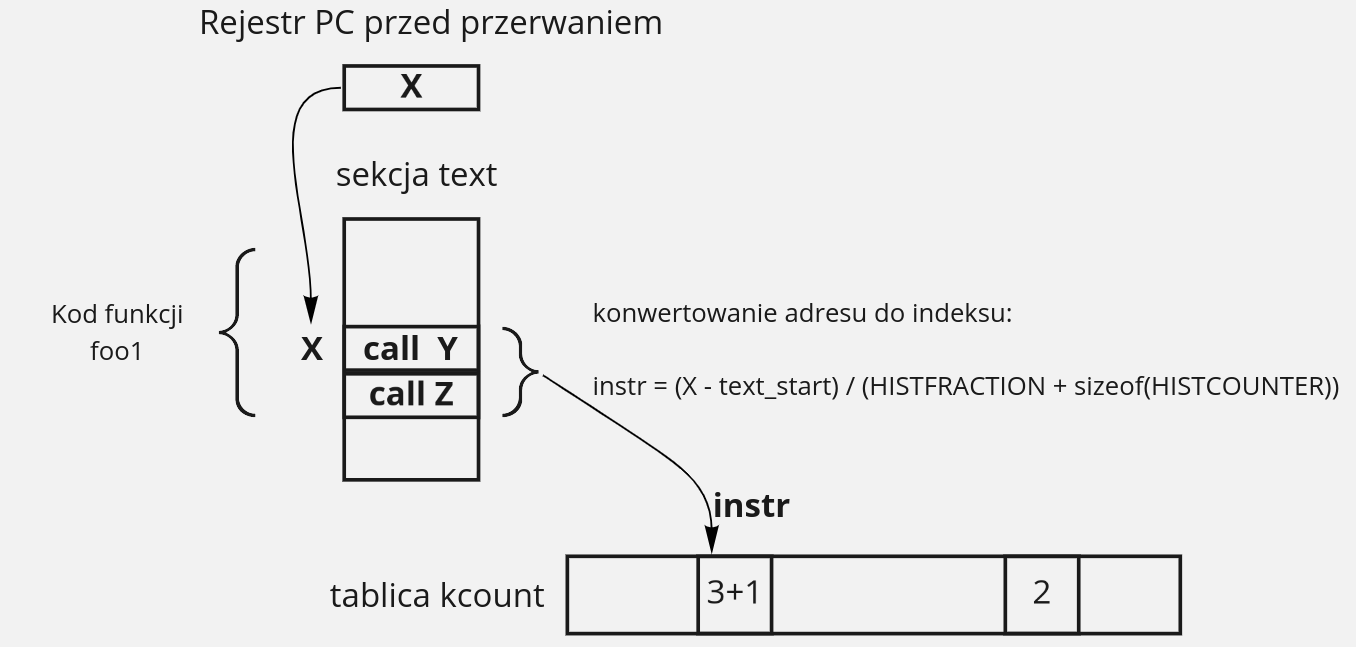
\includegraphics[scale=0.3]{images/kcount.png}
            \caption{Zobrazowanie zależności pomiędzy rejestrem PC, a sekcją text oraz tablicą kcount, a sekcją text}
        \end{figure}
        Podczas powyższego przykładu próbkowania adres przerwanej funkcji otrzymujemy z rejestru PC (ang. program counter) w momencie przed przerwaniem, następnie obliczany jest numer kubełka (instr), do którego należy adres. Pod koniec zwiększamy liczbę próbkowań dla tego kubełka (3+1).
    \item \textbf{kcountsize} rozmiar pamięciowy tablicy kcount
    \item \textbf{froms} tablica wskazująca na początek listy wołanych funkcji (w tablicy tos) przez pewną funkcję (z pewnego kubełka adresów).
        \begin{figure}[H]
            \centering
            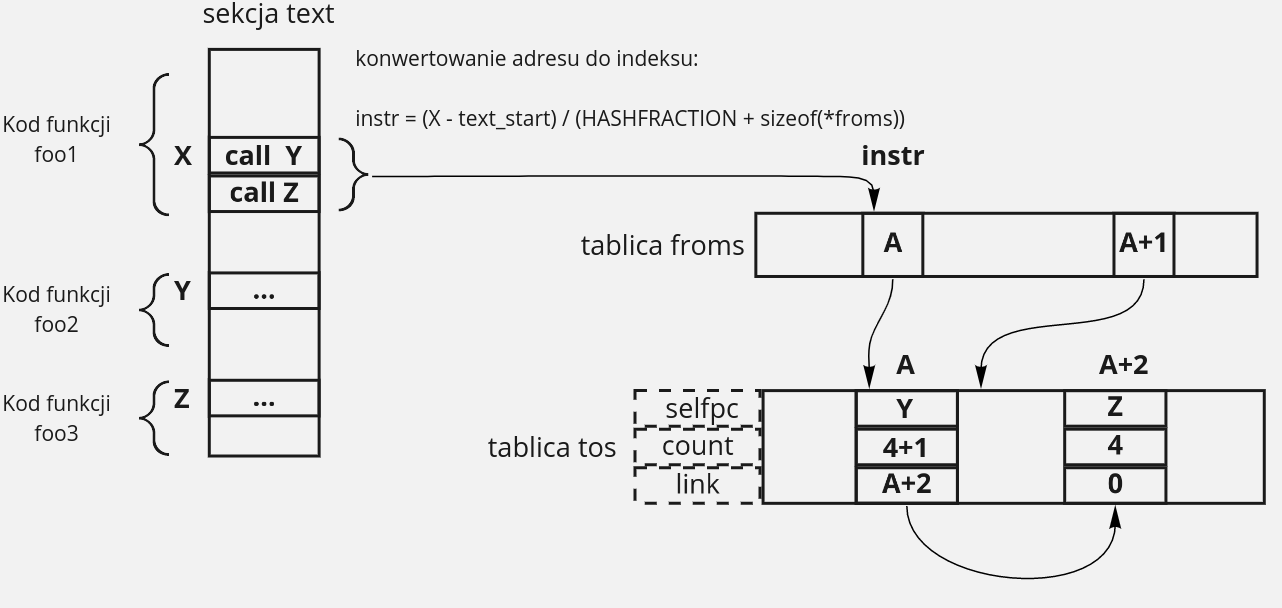
\includegraphics[scale=0.3]{images/froms.png}
            \caption{Zobrazowanie zależności pomiędzy strukturami froms i tos, a także skcją text i froms}
        \end{figure}
     W powyższym przykładzie mamy zobrazowany stan struktury froms i tos dla funkcji foo1, która w swoim kodzie woła funkcje foo2 i foo3. W sytuacji na obrazku aktualnie wykonana została instrukcja X, która woła funkcję foo2 (adres Y). Przed wywołaniem wykonywana jest funkcja instrumentująca kod i zwiększająca licznik wywołań funkcji zaczynającej się od adresu Y dla kubełka instr. Warto zwrócić uwagę, że w powyższym przykładzie do kubełka trafiają dwie instrukcje wywołujące inne funkcje przez co instr wskazuje na listę o dwóch węzłach.
    \item \textbf{fromssize} rozmiar pamięciowy tablicy froms
    \item \textbf{tos} wskaźnik na wcześniej wspomnianą tablicę to\_struct, która pozwala na tworzenie list wołanych funkcji (rozmiar jest procentowo zależny od rozmiaru sekcji text)
    \item \textbf{tossize} wielkość pamięciowa tablicy tos
    \item \textbf{tolimit} liczba węzłów tostruct\_t w tablicy tos
    \item \textbf{lowpc} początek sekcji text (najmniejszy adres)
    \item \textbf{highpc} koniec sekcji text (najmniejszy adres nie należący do text)
    \item \textbf{textsize} rozmiar sekcji text
    \item \textbf{hashfraction} dokładność kodowania przestrzeni adresowej text
\end{itemize}

Kgprof może przyjąć pięć stanów:

\begin{longlisting}
  \begin{minted}{c}
typedef enum {
  GMON_PROF_ON = 0,
  GMON_PROF_BUSY = 1,
  GMON_PROF_ERROR = 2,
  GMON_PROF_OFF = 3,
  GMON_PROF_NOT_INIT = 4,
} gmon_state_t;
  \end{minted}
  \caption{\href{https://mimiker.ii.uni.wroc.pl/source/xref/mimiker/include/sys/gmon.h?r=27b8c19a&mo=4347&fi=136\#136}{Typ wyliczeniowy gmon\_state\_t}}
  \label{lst:enumgmonstate}
\end{longlisting}

Stany te służą do sprawdzenia np. czy należy zbierać informacje, czy można odczytać spójne dane ze struktur:

\begin{itemize}
    \item \textbf{GMON\_PROF\_ON} - włączony
    \item \textbf{GMON\_PROF\_BUSY} - zajęty - dokonywane są aktualizacje na strukturach, flaga wykorzystywana jest, aby uzyskać spójne dane
    \item \textbf{GMON\_PROF\_ERROR} - błąd - zabrakło wolnych węzłów z tablicy tos
    \item \textbf{GMON\_PROF\_OFF} - wyłączony
    \item \textbf{GMON\_PROF\_NOT\_INIT} - nie zainicjalizowany
\end{itemize}

\subsection{Inicjalizacja profilera}

Podobnie jak w przypadku inicjalizacji zegara za pomocą \textbf{init\_clock} przed startem jądra w tej samej funkcji (init\_main) przygotowuje się profiler do działania za pomocą \textbf{init\_kgprof}.

\begin{longlisting}
  \begin{minted}{c}
/*
 * Structure prepended to gmon.out profiling data file.
 */
typedef struct gmonhdr {
  u_long lpc;   /* base pc address of sample buffer */
  u_long hpc;   /* max pc address of sampled buffer */
  int ncnt;     /* size of sample buffer (plus this header) */
  int version;  /* version number */
  int profrate; /* profiling clock rate */
  int spare[3]; /* reserved */
} gmonhdr_t;

#define GMONVERSION 0x00051879

/*
 * histogram counters are unsigned shorts (according to the kernel).
 */
typedef unsigned short HISTCOUNTER;

/*
 * fraction of text space to allocate for histogram counters here, 1/2
 */
#ifndef HISTFRACTION
#define HISTFRACTION 2
#endif /* HISTFRACTION */

#define INSTR_GRANULARITY HISTFRACTION * sizeof(HISTCOUNTER)

/* ... */

#define HASHFRACTION 2

/*
 * percent of text space to allocate for tostructs with a minimum.
 */
#define ARCDENSITY 2
#define MINARCS 50
#define MAXARCS ((1 << (unsigned int)(8 * sizeof(HISTCOUNTER))) - 2)

  \end{minted}
  \caption{Makra i \href{https://mimiker.ii.uni.wroc.pl/source/xref/mimiker/include/sys/gmon.h?r=27b8c19a\#47}{struktura gmonhdr\_t} wykorzystywana przy inicjalizacji profilera}
  \label{lst:structgmonhdr}
\end{longlisting}

Struktura \textbf{gmonhdr\_t} wykorzystywana jest do tworzenia pliku wyjściowego z zebranymi danymi naszego narzędzia. Przechowuje ona zakres adresów sekcji text -- \textbf{lpc} i \textbf{hpc}, rozmiar tablicy próbkującej (kcount) wraz z własnym rozmiarem -- \textbf{ncnt}, wersje profilera -- \textbf{version}, częstotliwość zegara próbkującego -- \textbf{profrate}, a także trzy inty zarezerwowane na przyszły rozwój narzędzia -- \textbf{spare}. Ta struktura pozwala na to, aby narzędzie analizujące te dane -- gprof wiedział w jaki sposób są one przechowywane.

Makra z końcówką \textbf{FRACTION} służą do konwertowania adresów funkcji na indeksy tablic - kcount i froms. Pozwala to na zaoszczędzenie pamięci przy alokacji tablic (kcount i froms), ponieważ np. instrukcje maszynowe zazwyczaj są oddalone w kodzie maszynowym o kilka bajtów. Dzięki temu nie potrzeba alokować tablic o takich samych wielkościach co rozmiar sekcji text, aby móc rozpoznawać, która komórka odpowiada danemu wywołaniu. Dlatego właśnie stosuje się pewien rodzaj kompresji, gdzie np. adres x jest konwertowany do indeksu tablicy froms (x -  początek\_sekcji\_text) / (HASHFRACTION + sizeof(*froms)), a odwrócenie tego procesu dla intów daje tylko HASHFRACTION + sizeof(*froms) kandydatów z czego zazwyczaj tylko jeden jest prawidłowy. Dodatkowo

\textbf{HISTFRACTION} odpowiada jaki ułamek wielkości sekcji text chcemy użyć do jej zakodowania dla tablicy kcount, wykorzystywanej do próbkowania funkcji za pomocą zegara. \textbf{HASHFRACTION} działa podobnie, lecz odnosi się do zakodowania przestrzeni text, aby rozpoznawać skąd jest wywoływana funkcja (potrzebne do tworzenia grafu wywołań). \textbf{ARCDENSITY} oznacza jaki procent sekcji text chcemy alokować dla struktur tostruct\_t, inaczej ile węzłów dla naszych list chcemy przygotować w zależności od rozmiaru sekcji.

Makro HISTCOUNTER odpowiada za typ tablicy kcount.

\begin{longlisting}
  \begin{minted}{c}
void init_kgprof(void) {
  gmonparam_t *p = &_gmonparam;

  @\llabel{kgprofset}@p->lowpc = rounddown((u_long)__text, INSTR_GRANULARITY);
  p->highpc = roundup((u_long)__etext, INSTR_GRANULARITY);
  p->textsize = p->highpc - p->lowpc;
  p->kcountsize = p->textsize / HISTFRACTION;
  p->hashfraction = HASHFRACTION;
  p->fromssize = p->textsize / HASHFRACTION;
  p->tolimit = (p->textsize * ARCDENSITY) / 100;
  p->tolimit = min(max(p->tolimit, MINARCS), MAXARCS);
  p->tossize = p->tolimit * sizeof(tostruct_t);

  @\llabel{kgprofalloc}@size_t size = p->kcountsize + p->tossize + p->fromssize;
  void *profptr = kmem_alloc(align(size, PAGESIZE), M_NOWAIT | M_ZERO);
  assert(profptr != NULL);

  p->tos = (tostruct_t *)profptr;
  profptr += p->tossize;
  p->kcount = (u_short *)profptr;
  profptr += p->kcountsize;
  p->froms = (u_short *)profptr;

  assert(is_aligned(p->tos, alignof(tostruct_t)));
  assert(is_aligned(p->kcount, alignof(u_short)));
  assert(is_aligned(p->froms, alignof(u_short)));

  @\llabel{kgprofhdr}@gmonhdr_t *hdr = &_gmonhdr;
  hdr->lpc = p->lowpc;
  hdr->hpc = p->highpc;
  hdr->ncnt = p->kcountsize + sizeof(gmonhdr_t);
  hdr->version = GMONVERSION;
  hdr->spare[0] = hdr->spare[1] = hdr->spare[2] = 0;

  p->state = GMON_PROF_ON;
}
  \end{minted}
  \caption{\href{https://mimiker.ii.uni.wroc.pl/source/xref/mimiker/sys/kern/kgprof.c?r=27b8c19a\#12}{Funkcja init\_kgprof}}
  \label{lst:funcinitkgprof}
\end{longlisting}

Najpierw ustawia się wszystkie parametry związane z sekcją text \ref{kgprofset} -  dolna (\_\_text to pierwszy adres sekcji text) i górna (\_\_etext to pierwszy adres poza sekcją)  granica sekcji z zaokrągleniem do ziarnistości (gęstości) zbierania danych. Pozwala to na ominięcie problemu zaokrąglania w dół w przypadku dzielenia (p$\rightarrow$textsize / HISTFRACTION), a następnie wielkości wszystkich struktur potrzebnych do przechowywania danych (mają one stały rozmiar w pamięci).

Następnie oblicza się jakiej wielkości blok pamięci jest potrzebny do przechowywania wszystkich struktur, alokuje blok pamięci i odpowiednio przypisuje wskaźniki dla każdej struktury \ref{kgprofalloc}.

Ostatnim etapem jest wypełnienie struktury \textbf{gmonhdr\_t} (wykorzystywana do tworzenia pliku wyjściowego profilera) i zmiana stanu profilera na uruchomiony \ref{kgprofhdr}.

\subsection{Instrumentacja}

Aby umożliwić instrumentację, a także profilowanie w naszym systemie należy go skompilować z flągą \textbf{KGPROF=1}, gdzie podczas budowania ustawia się odpowiednie opcje:


\begin{longlisting}
  \begin{minted}{make}
ifeq ($(KGPROF), 1)
    CFLAGS_KGPROF = -finstrument-functions
endif
  \end{minted}
  \caption{\href{https://mimiker.ii.uni.wroc.pl/source/xref/mimiker/build/arch.mips.mk?r=27b8c19a\#28}{Fragment skryptu dla make -- arch.mips.mk}}
  \label{lst:makefile}
\end{longlisting}

Wykorzystując opcję kompilatora gcc \textbf{-finstrument-functions} \cite{bib:gccflags} generuje ona instrumentację wywołując funkcje przed i po wywoływaniu instrumentowanej funkcji. Wywoływanymi funkcjami są odpowiednio  \textbf{\_\_cyg\_profile\_func\_enter} oraz  \textbf{\_\_cyg\_profile\_func\_exit}. Funkcje przyjmują dwa argumenty: adres wołanej funkcji oraz skąd wołana jest funkcja. Na potrzeby profilera potrzebna jest nam tylko jedna funkcja, dlatego przedstawimy \_\_cyg\_profile\_func\_enter, gdyż druga funkcja pozostaje pusta i wymagana jest tylko jej deklaracja na potrzeby istnienia jej symbolu podczas kompilacji. Flaga na potrzeby systemu jest włączona tylko dla kodu znajdującego się w jądrze, dlatego instrumentacji nie ulegną funkcje spoza sekcji text przeznaczonej dla jądra.

\begin{longlisting}
\begin{minted}{c}
__no_profile void __cyg_profile_func_enter(void *self, void *from) {
  u_long frompc = (u_long)from, selfpc = (u_long)self;
  u_short *frompcindex;
  tostruct_t *top, *prevtop;
  gmonparam_t *p = &_gmonparam;
  long toindex;

 @\llabel{profilernoton}@if (p->state != GMON_PROF_ON)
    return;

   @\llabel{profilelock}@WITH_SPIN_LOCK (&mcount_lock) {
    /*
     * To ensure consistent data in kgmon - this function can move
     * a node from the middle of the list to the beginning and
     * during this process we can omit it while accesing the structure.
     */
    p->state = GMON_PROF_BUSY;
    /*
     * check that frompc is a reasonable pc value.
     * for example:	signal catchers get called from the stack,
     *		not from text space.  too bad.
     */
    @\llabel{profilefrompc}@frompc -= p->lowpc;
    if (frompc >= p->textsize)
      goto done;

    @\llabel{profilefrominedx}@size_t index = (frompc / (HASHFRACTION * sizeof(*p->froms)));
    frompcindex = &p->froms[index];
    toindex = *frompcindex;
    /*
     *	First time profiling this calling function .
     */
    @\llabel{profiletoindex0}@if (toindex == 0) {
      /*
       * Getting an unused node (the smallest unused tos entry index).
       */
      toindex = ++p->tos[0].link;
      if (toindex >= p->tolimit) {
        p->state = GMON_PROF_ERROR;
        goto done;
      }

      *frompcindex = (u_short)toindex;
      top = &p->tos[(size_t)toindex];
      top->selfpc = selfpc;
      top->count = 1;
      top->link = 0;
      goto done;
    }
    @\llabel{profileliststart}@top = &p->tos[(size_t)toindex];
    /*
     * Node with our called function at front of chain; usual case.
     */
    if (top->selfpc == selfpc) {
      top->count++;
      goto done;
    }
    /*
     * Traversing the list and looking for node with our called function.
     */
    while (true) {
      /*
       * We reached the end of the list it does not contain a node with
       * the called function. Check if there are still available nodes to use,
       *  if so get one and add it to the list.
       */
      @\llabel{profilelistend}@if (top->link == 0) {
        toindex = ++p->tos[0].link;
        if (toindex >= p->tolimit) {
          p->state = GMON_PROF_ERROR;
          goto done;
        }

        top = &p->tos[(size_t)toindex];
        top->selfpc = selfpc;
        top->count = 1;
        top->link = *frompcindex;
        *frompcindex = (u_short)toindex;
        goto done;
      }
      /*
       * Move to the next node.
       */
      prevtop = top;
      top = &p->tos[top->link];
      /*
       * We found our node,remove it from our list
       * and add it at the beginning of the list.
       */
      @\llabel{profilelistnextcheck}@if (top->selfpc == selfpc) {
        top->count++;
        toindex = prevtop->link;
        prevtop->link = top->link;
        top->link = *frompcindex;
        *frompcindex = (u_short)toindex;
        goto done;
      }
    }
  @\llabel{profiledone}@done:
    if (p->state != GMON_PROF_ERROR)
      p->state = GMON_PROF_ON;
  }
}
\end{minted}
  \caption{\href{https://mimiker.ii.uni.wroc.pl/source/xref/mimiker/sys/kern/mcount.c?r=27b8c19a&mo=4721&fi=98\#98}{Funkcja \_\_cyg\_profile\_func\_enter}}
  \label{lst:funccygprofileenter}
\end{longlisting}

Funkcja najpierw odczytuje odpowiednie wartości, a następnie sprawdza czy profilowanie jest włączone \ref{profilernoton}.

W przypadku włączonego narzędzia blokada wirująca jest zakładana do końca działania funkcji \ref{profilelock} i oznacza profiler jako zajęty gdyż zmieniane są dane i chcemy zapewnić, że podczas tej operacji nie dokonamy innej zmiany w tym samym czasie. Następnie oblicza się adres funkcji względem początku sekcji text oraz sprawdza się  czy należy do tej sekcji \ref{profilefrompc} (procedura powrotu z sygnału jest umieszczana na stosie). Dalej koduje się miejsce skąd wołana jest funkcja \ref{profilefrominedx}, odczytuje się wskazanie na pierwszy węzeł w liście wołanych funkcji (indeks tablicy tos) przez ten kod. 

Wartość zero oznacza, że z tego miejsca jeszcze nie była wołana żadna funkcja \ref{profiletoindex0} przez co z tablicy tos otrzymujemy indeks, pierwszego wolnego węzła tablicy, który jest przechowywany pod indeksem - tos[0].link + 1. Jeśli indeks wykracza poza tablicę oznaczamy wystąpienie błędu i wykonujemy skok bezwarunkowy do done, w przeciwnym przypadku wypełniamy pola struktury oraz oznaczamy, że jest to ostatni element listy (top$\rightarrow$link = 0) i skaczemy do done.

Jeśli wartość nie jest zerowa, czyli lista nie jest pusta odczytujemy jej pierwszy węzeł \ref{profileliststart} i sprawdzamy czy zawiera informacje o naszej funkcji, jeśli tak to zwiększamy licznik wywołań i przechodzimy do done. Jeśli warunek nie został spełniony przechodzimy listę, dopóki:
\begin{enumerate}
    \item nie natrafimy na koniec \ref{profilelistend} i w trakcie postępujemy podobnie jak poprzednio.
    \item natrafimy na węzeł, który zawiera naszą funkcję \ref{profilelistnextcheck} i postępujemy jak poprzednio wraz z dodaniem tego węzła na początek listy (wynika to z lokalności wywołań, gdzie z większym prawdopodobieństwem wywołamy z tego miejsca funkcję, którą ostatnio wołaliśmy).
\end{enumerate}

Pod koniec w done oznaczamy, że profiler nie jest już zajęty.

Warto zwrócić uwagę, że przy deklaracji funkcji jest atrybut \textbf{\_\_no\_profile}, który jest pośrednim makrem na \textbf{\_\_attribute\_\_((no\_instrument\_function))}. Jest on kluczowy, ponieważ w przeciwnym przypadku funkcja ta podlegałaby też instrumentacji i powstałaby nieskończona rekursja. Należy pamiętać, aby funkcje, które są wykorzystywane w instrumentach też nie podlegały temu procesowi (funkcje wykonywane pomiędzy sprawdzeniem czy profiler jest włączony, a oznaczeniem, że jest zajęty) np. funkcja włączająca przerwania z tego powodu nie jest instrumentowana. W jądrze istnieją też funkcje, które mają pewne założenia na temat stosu lub przechowywanych wartości w rejestrach przez funkcje wołające, jeśli zostałaby wywołana funkcja instrumentująca przed taką funkcją to założenia te mogłyby nie zostać spełnione. Takie funkcje też nie są profilowane, w Mimikerze jest to np. \textbf{copystr}.

\subsection{Próbkowanie}

Narzędzie również stosuje próbkowanie systemu, aby oszacować ile czasu procesora wykorzystywała funkcja \cite{bib:kgprofprofclock}. Jeśli jest taka możliwość inicjalizuje się dodatkowy zegar, który służy do obsługi próbkowania, w przypadku kiedy nie mamy osobnego zegara, rutynę tą obsługuje zegar systemowy. Funkcją wołaną przez zegar jest \textbf{kgprof\_tick}.

\begin{longlisting}
  \begin{minted}{c}
void kgprof_tick(void) {
  assert(intr_disabled());

  uintptr_t pc, instr;
  gmonparam_t *g = &_gmonparam;
  @\llabel{kgprofthread}@thread_t *td = thread_self();

  @\llabel{kgprofinkern}@if (td->td_kframe == NULL)
    return;

  pc = ctx_get_pc(td->td_kframe);
  @\llabel{kgproftickcheck}@if (g->state == GMON_PROF_ON && pc >= g->lowpc) {
    instr = pc - g->lowpc;
    if (instr < g->textsize) {
      instr /= INSTR_GRANULARITY;
      g->kcount[instr]++;
     }
  }
}
  \end{minted}
  \caption{\href{https://mimiker.ii.uni.wroc.pl/source/xref/mimiker/sys/kern/kgprof.c?r=27b8c19a\#49}{Funkcja kgrof\_tick}}
  \label{lst:funckgproftck}
\end{longlisting}

Najpierw odczytujemy strukturę gmonparam\_t oraz thread\_t aktualnego wątku \ref{kgprofthread}, druga struktura pozwala nam uzyskać dostęp do 'obrazu' jądra, czyli kontekstu wątku przed wystąpieniem przerwania.
Jeśli wątek nie był w jądrze wracamy \ref{kgprofinkern}, w przeciwnym przypadku odczytujemy z zapisanego kontekstu rejestr PC , który wskazuje na wykonywaną instrukcję. Następnie sprawdzamy czy profiler jest włączony, a także czy PC jest z odpowiedniego przedziału \ref{kgproftickcheck}, a następnie skaluje się odpowiednio adres i zlicza czas wykonania dla poprzednio działającej funkcji w tablicy kcount.

\section{Kgmon}

Aby wykorzystać zebrane dane potrzebne było narzędzie, które umożliwi pobranie tych informacji, System do niedawna był tylko możliwy do uruchomienia pod emulacją wraz ze wsparciem GDB i jego skryptowaniem w Pythonie \cite{bib:gdb-python}. Dlatego wybrałem implementację funkcji dla tego właśnie debuggera. We FreeBSD korzysta się z podobnego narzędzia, lecz z dostępem do większej liczby opcji, a także możliwością bezpośredniego użycia z profilowanej maszyny \cite{bib:freebsdkgmon}.

\begin{longlisting}
  \begin{minted}{python}
class Kgmon(SimpleCommand):
    """Dump the gprof data to file (by default 'gmon.out')"""

    def __init__(self):
        super().__init__('kgmon')

    def __call__(self, args):
        args = args.strip()
        state = gdb.parse_and_eval('_gmonparam.state')
        if state == gdb.parse_and_eval('GMON_PROF_NOT_INIT'):
            print("Kgprof not initialized yet")
        elif state == gdb.parse_and_eval('GMON_PROF_BUSY'):
            # To ensure consistent data
            print("The mcount function is running - wait for it to finish")
        else:
            if state == gdb.parse_and_eval('GMON_PROF_ERROR'):
                print("The tostruct array was too small for the whole process")
            gmon_write(args or 'gmon.out')

  \end{minted}
  \caption{\href{https://mimiker.ii.uni.wroc.pl/source/xref/mimiker/sys/debug/kgmon.py?r=624198e4\#56}{Implementacja komendy kgmon dla gdb}}
   \label{lst:funckgmon}
\end{longlisting}

Powyższa funkcja definiuje komendę kgmon dla gdb. Komenda służy do zapisania zebranych danych do pliku wyjściowego (domyślnie do pliku gmon.out, chyba, że zostanie podany argument do jakiego pliku mają zostać zapisane dane). Odczytuje stan profilera oraz sprawdza czy został już zainicjalizowany oraz czy mamy zapewnienie o spójności danych. Jeśli oba warunki zostały spełnione to dokonuje się odczytu danych za pomocą funkcji \textbf{gmon\_write}, w przeciwnym przypadku wyświetla się odpowiedni komunikat błędu.

\begin{longlisting}
  \begin{minted}{python}
  def gmon_write(path):
    class GmonParam(metaclass=GdbStructMeta):
        __ctype__ = 'struct gmonparam'

    gparam = GmonParam(gdb.parse_and_eval('_gmonparam'))
    infer = gdb.inferiors()[0]

    with open(path, "wb") as of:
        # Write headers
        gmonhdr_size = int(gdb.parse_and_eval('sizeof(_gmonhdr)'))
        gmonhdr_p = gdb.parse_and_eval('&_gmonhdr')
        of.write(infer.read_memory(gmonhdr_p, gmonhdr_size))

        # Write tick buffer
        of.write(infer.read_memory(gparam.kcount, gparam.kcountsize))

        # Write arc info
        memory = infer.read_memory(gparam.froms, gparam.fromssize)
        froms_array = unpack('H' * int(gparam.fromssize/calcsize('H')), memory)
        memory = infer.read_memory(gparam.tos, gparam.tossize)

        # The last H stands for padding in the tos strusture
        tos_rep = 'IiHH'
        tos_rep_len = len(tos_rep)
        size = calcsize(tos_rep)
        tos_array = unpack(tos_rep * int(gparam.tossize/size), memory)

        fromindex = -1
        froms_el_size = int(gdb.parse_and_eval('sizeof(*_gmonparam.froms)'))
        for from_val in froms_array:
            fromindex += 1
            # Nothing has been called from this function
            if from_val == 0:
                continue
            # Getting the calling function addres from encoded value
            offset = fromindex * froms_el_size * gparam.hashfraction
            frompc = gparam.lowpc + offset
            toindex = from_val

            # Traversing the tos list for the calling function
            # It stores data about called functions
            while toindex != 0:
                selfpc = tos_array[toindex * tos_rep_len]
                count = tos_array[toindex * tos_rep_len + 1]
                toindex = tos_array[toindex * tos_rep_len + 2]
                of.write(pack('IIi', frompc, selfpc, count))
  \end{minted}
  \caption{\href{https://mimiker.ii.uni.wroc.pl/source/xref/mimiker/sys/debug/kgmon.py?r=624198e4\#8}{Funkcja gmon\_write}}
  \label{lst:funcgmonwrite}
\end{longlisting}

Standardowy skrypt Pythonowy dla kgmona. Odczytuje strukturę \textbf{\_gmonparam} i wykorzystuje infrastrukturę gdb do szybkiego odczyt pamięci \cite{bib:inferior}. Następnie otwierany jest plik, do którego odbyć ma się zapis i zapisuje się według ściśle określonej kolejności:

\begin{enumerate}
    \item informacje zawarte w \textbf{\_gmonhdr}
    \item całą tablicę \textbf{kcount}
    \item \textbf{krawędzie grafu wywołań} w postaci funkcja wołająca, funkcja wołana i liczba wywołań
\end{enumerate}

Plik wyjściowy w takim formacie umożliwi jego przetworzenie za pomocą gprofa.

\section{Profilowanie systemu Mimiker}

Aby umożliwić profilowanie w naszym systemie należy skompilować system z flagą \textbf{KGPROF=1}:

\begin{listing}[H]
  \begin{minted}{bash}
    > make KGPROF=1
\end{minted}
  \label{lst:makekgprofmimiker}
\end{listing}


Po kompilacji, można uruchomić program z debuggerem (-d) w dowolnym trybie np. sprawdzenia testów:

\begin{listing}[H]
  \begin{minted}{bash}
    > ./launch -d test=all
\end{minted}
  \label{lst:launchtestmimiker}
\end{listing}

Za pomocą debuggera GDB najpierw należy kontynuować działanie programu, a następnie w dogodnym momencie (pomijając moment wykonywania kodu instrumentującego) należy wywołać komendę \textbf{kgmon [nazwa\_pliku\_wyjściowego]}.


\begin{listing}[H]
  \begin{minted}{bash}
    (gdb) kgmon
\end{minted}
  \label{lst:dumpmimiker}
\end{listing}

Plik wyjściowy gotowy jest już do przetwarzania, ale niezbędne jest podanie pliku wykonywalnego z obrazem systemu, aby komenda potrafiła powiązać symbole wraz z zebranymi danymi.

\begin{listing}[H]
  \begin{minted}{bash}
    > gprof sys/mimiker.elf gmon.out | less
\end{minted}
  \label{lst:gprodmimiker}
\end{listing}

W ten sposób otrzymujemy wcześniej opisane wyniki profilowania:

\begin{longlisting}
  \begin{minted}{c}
  Flat profile:

Each sample counts as 0.000274499 seconds.
  %   cumulative   self              self     total           
 time   seconds   seconds    calls  ms/call  ms/call  name    
 70.12      9.12     9.12                             cpu_intr_enable
  6.26      9.94     0.81                             __cyg_profile_func_enter
  3.04     10.33     0.40                             _spin_lock
  2.91     10.71     0.38    18381     0.02     0.02  bzero
  2.26     11.01     0.29                             spin_unlock
  1.76     11.24     0.23                             intr_enable
  1.71     11.46     0.22   379329     0.00     0.00  mtx_owned
  1.08     11.60     0.14                             bcopy
  1.08     11.74     0.14                             intr_disable
  0.91     11.86     0.12   168245     0.00     0.00  _mtx_lock
  0.75     11.96     0.10   168245     0.00     0.00  mtx_unlock
  0.59     12.03     0.08        1    77.41    77.50  test_kmem
  0.53     12.10     0.07                             __cyg_profile_func_exit
  0.53     12.17     0.07                             memcpy
  0.48     12.23     0.06    10500     0.01     0.03  pool_alloc
  0.40     12.28     0.05                             thread_self
  0.30     12.32     0.04      334     0.12     0.15  pmap_add_pde
  0.29     12.36     0.04    29323     0.00     0.00  pmap_extract_nolock
  0.26     12.39     0.03                             cpu_intr_disable
  0.24     12.43     0.03    22620     0.00     0.00  vm_page_find
  0.23     12.46     0.03        1    30.47    30.47  sched_run
  0.20     12.48     0.03     7475     0.00     0.01  vm_object_add_page
  0.19     12.51     0.02    51895     0.00     0.00  klog_append
  \end{minted}
  \caption{Wynik płaskiego profilowania dla testów w Mimikerze}
  \label{lst:flatprofmimiker}
\end{longlisting}

Wyniki dla pierwszych funkcji są zniekształcone, ponieważ przerwanie z zegara profilującego może przyjść w trakcie działania funkcji z wyłączonymi przerwaniami i podczas ich ponownego włączania zostanie obsłużone, przez co tak często trafiamy np. cpu\_intr\_enable.

\begin{longlisting}
  \begin{minted}{c}
                       Call graph (explanation follows)


granularity: each sample hit covers 4 byte(s) for 0.00% of 13.01 seconds

index % time    self  children    called     name
                                                 <spontaneous>
[1]     70.1    9.12    0.00                 cpu_intr_enable [1]
-----------------------------------------------
                                                 <spontaneous>
[2]     12.6    0.00    1.63                 mips_exc_handler [2]
                0.00    0.98    4533/4533        user_trap_handler [3]
                0.00    0.65    9635/9635        kern_trap_handler [9]
-----------------------------------------------
                0.00    0.98    4533/4533        mips_exc_handler [2]
[3]      7.6    0.00    0.98    4533         user_trap_handler [3]
                0.00    0.83    2422/2422        syscall_handler [4]
                0.00    0.14    2103/11738       tlb_exception_handler [6]
                0.00    0.01    4424/4510        on_user_exc_leave [136]
                0.00    0.00    4424/64557       on_exc_leave [125]
                0.00    0.00    4533/82618       preempt_disabled [134]
                0.00    0.00       4/23          sig_trap [533]
                0.00    0.00     144/144         __cleanup_proc_unlock [1892]
                0.00    0.00       4/23          __cleanup_mtx_unlock [1904]
                0.00    0.00       4/23          mtx_lock [1110]
-----------------------------------------------
  \end{minted}
  \caption{Graf wywołań dla testów w Mimikerze}
  \label{lst:callgraphmimiker}
\end{longlisting}
\chapter{Podsumowanie}

Praca nad systemem Mimiker pozwoliła mi zgłębić wiedzę na temat działania jądra systemu operacyjnego. Mimo skupienia się na dwóch tematach --- infrastrukturze czasu i profilowaniu, to obszarów, z którymi miałem styczność jest znacznie więcej, m.in. wcześniej wspomniane schedulery. To właśnie podczas analizowania schedulera ULE występującego w jądrze systemu FreeBSD natrafiłem na niekonsekwentny opis funkcji obliczającej priorytet wątku, co po przeanalizowaniu kodu pozwoliło na wniesienie poprawki do opisu tej funkcji.

Podczas pracy nad infrastrukturą czasu dostarczyłem wywołania systemowe - gettimeofday i nanosleep. Wywołania te umożliwiły działanie komendy date, zapis  czasu utworzenia plików w systemie czy funkcji sleep, którą wykorzystuje się w Mimikerze m.in. przy nieudanych próbach logowania dla komendy login. Ujednoliciłem stosowanie struktury bintime\_t w jądrze, co wyeliminowało niepotrzebne konwersje między reprezentacjami i uprościło kod jądra. Zaimplementowałem działający zegar PIT. Pozwoliło to na korzystanie z dwóch działających zegarów w naszym systemie. Dzięki temu możemy drugi zegar wykorzystywać do próbkowania asynchronicznego względem naszego zegara systemowego.

Próbkowanie asynchroniczne było ważne, aby móc dostarczyć w pełni działające narzędzie kgprof dla naszego systemu. 
Dostarczony przeze mnie profiler pozwala na zobrazowanie działania systemu poprzez informacje na temat liczby wywołań funkcji, grafu wywołań czy estymację czasu działania funkcji. Narzędzie umożliwia nam badanie systemu za pomocą własnego dedykowanego zegara.

\section{Dalsza praca}

Projekt oferuje wiele możliwości do dalszego rozwoju. Poczynając od rozbudowy infrastruktury czasu po wykorzystanie profilera do analizy wydajności systemu, a następnie jego optymalizacji, na rozwoju samego narzędzia kończąc.

W infrastrukturze czasu nie mamy wsparcia dla zmiany czasu zegarowego (ang. wall time) podczas działania systemu, implementacja wywołania systemowego settimeofday umożliwiłaby takie manipulacje. Samą infrastrukturę można zoptymalizować wyeliminowując zakładanie blokad podczas odczytu czasu, np. za pomocą pierścienia opisanego w rozdziale 2.

Nasze narzędzie do profilowania zbiera informacje tylko dla jądra systemu Mimiker. Można przystosować infrastrukturę zegara próbkującego, aby działała tylko podczas pracy w trybie jądra, czyli np. włączać zegar tylko podczas pobytu w jądrze.

Istnieją pomysły na zwiększenie wiarygodności estymowania czasu działania funkcji, a także na uniknięcie zsynchronizowania się programów z profilerem poprzez losowanie okresu pomiędzy próbkowaniami. Ta idea została opisana w pracy \cite{bib:randomizedgprof}, gdzie przedstawiono korzystanie z ograniczonego losowania okresu tyknięć podczas próbkowania \cite{bib:randomizedgprof}, co pozwoli na lepsze mierzenie czasu działania funkcji oraz wyeliminowanie synchronizacji z zegarem próbkującym. 

Dla naszego narzędzia profilującego można sprawdzić jakie będą zbierane dane jeśli będziemy losowali okres próbkowania, przy wykorzystaniu zegara w trybie jednostrzałowym i w zależności od wylosowanego okresu przypisywać takiemu próbkowaniu odpowiednie wagi.

%%%%% BIBLIOGRAFIA

\begin{thebibliography}{100}

\bibitem{bib:Mimiker}
\textit{Projekt Mimiker},
\url{https://Mimiker.ii.uni.wroc.pl/}

\bibitem{bib:timecounters}
\textsc{Poul-Henning Kamp},
\textit{Timecounters: Efficient and precise timekeeping in SMP kernels}

\bibitem{bib:gprof}
\textsc{Susan L. Graham, Peter B. Kessler. Marshall K. McKusick},
\textit{gprof: a Call Graph Execution Profiler}

\bibitem{bib:fisr}
\textsc{Chris Lomont},
\textit{Fast Inverse Square Root}

\bibitem{bib:ule}
\textsc{Jeff Roberson},
\textit{ULE: A Modern Scheduler For FreeBSD}

\bibitem{bib:randomizedgprof}
\textsc{Steven Mccanne , Chris Torek},
\textit{A Randomized Sampling Clock for CPU Utilization Estimation and Code Profiling}

\bibitem{bib:callendarqueue}
\textsc{R. Brown},
\textit{Calendar queues: a fast 0(1) priority queue implementation for the simulation event set problem}

\bibitem{bib:jpszcz}
\textsc{Julian Pszczołowski},
\textit{Przegląd metod synchronizacji w jądrach systemów uniksopodobnych oraz implementacja rogatek w systemie operacyjnym Mimiker}


\bibitem{bib:lpi}
\textsc{Michael KerrisK},
\textit{The Linux Programming Interface}
No Starch Press, 2010.

\bibitem{bib:freebsd-os}
\textsc{Marshall Kirk McKusick, George V. Neville-Neil },
\textit{The Design And Implementation Of The Freebsd Operating System}
wyd. 2, Addison-Wesley Professional, 2014

\bibitem{bib:apue}
\textsc{W. Richard Stevens, Stephen A. Rago},
\textit{Advanced Programming in the UNIX Environment}
wyd. 3, Addison-Wesley Professional, 2013

\bibitem{bib:leapsec}
\textsc{Derick Rethans},
\textit{php|architect’s Guide to Date and Time Programming}
musketeers.me, 2009

\bibitem{bib:unp}
\textsc{W. Richard Stevens, Bill Fenner, Andrew M. Rudoff},
\textit{Unix Network Programming: The Sockets Networking API}
Addison-Wesley Professional, 2003

\bibitem{bib:lkd}
\textsc{Robert Love},
\textit{Linux Kernel Development},
wyd. 3, Addison-Wesley Professional, 2010.

\bibitem{bib:denis}
\textsc{Denis Bakhvalo},
\textit{Performance Analysis and Tuning on Modern CPUs},
2020.

\bibitem{bib:rtc}
\textit{mc146818 RTC},
\url{https://www.e-merchan.com/media/pdf/MC146818.pdf}

\bibitem{bib:pit}
\textit{Intel manual},
\textit{8254 Programmable Interval Timer},
\url{https://www.scs.stanford.edu/10wi-cs140/pintos/specs/8254.pdf}

\bibitem{bib:ccnt}
\textit{CCNT ARM11},
\url{https://developer.arm.com/documentation/ddi0360/f/control-coprocessor-cp15/register-descriptions/c15--cycle-counter-register--ccnt-}

\bibitem{bib:perf}
\textit{Perf wiki},
\url{https://perf.wiki.kernel.org/index.php/Main_Page}

\bibitem{bib:vtune}
\textit{VTune},
\url{https://software.intel.com/content/www/us/en/develop/tools/oneapi/components/vtune-profiler.html#gs.9lp14y}

\bibitem{bib:gprof-out}
\textit{Gprof output description},
\url{https://ftp.gnu.org/old-gnu/Manuals/gprof-2.9.1/html_chapter/gprof_5.html}

\bibitem{bib:tm_t}
\textit{GNU libc manual},
\textit{Broken-down Time},
\url{https://www.gnu.org/software/libc/manual/html_node/Broken_002ddown-Time.html}

\bibitem{bib:time-types}
\textit{GNU libc manual},
\textit{Time-Types},
\url{https://www.gnu.org/software/libc/manual/html_node/Time-Types.html}

\bibitem{bib:kasan}
\textit{KASAN},
\url{https://www.kernel.org/doc/html/v4.14/dev-tools/kasan.html}

\bibitem{bib:kcsan}
\textit{KCSAN},
\url{https://www.kernel.org/doc/html/latest/dev-tools/kcsan.html}

\bibitem{bib:lockdep}
\textit{LOCKDEP},
\url{https://www.kernel.org/doc/Documentation/locking/lockdep-design.txt}

\bibitem{bib:rwlock}
\textit{Read/Wrtie locks},
\url{https://www.freebsd.org/cgi/man.cgi?query=rwlock&sektion=9&manpath=FreeBSD+7.1-RELEASE}

\bibitem{bib:calloutbsd}
\textit{Callout manual},
\url{https://www.freebsd.org/cgi/man.cgi?query=callout&sektion=9}

\bibitem{bib:freebsdkgmon}
\textit{Kgmon manual},
\url{https://www.freebsd.org/cgi/man.cgi?query=kgmon&apropos=0&sektion=0&manpath=FreeBSD+7.1-RELEASE&format=html}

\bibitem{bib:gprof-manual}
\textit{Gprof manual},
\url{https://man7.org/linux/man-pages/man1/gprof.1.html}

\bibitem{bib:gettime-manual}
\textit{Gettimeofday manual},
\url{https://man7.org/linux/man-pages/man2/settimeofday.2.html}

\bibitem{bib:clock_gettime}
\textit{Clock\_gettime manual},
\url{https://man7.org/linux/man-pages/man2/clock_getres.2.html}

\bibitem{bib:nanosleep-manual}
\textit{Nanosleep manual},
\url{https://man7.org/linux/man-pages/man2/nanosleep.2.html}

\bibitem{bib:clock_nanosleep}
\textit{Clock\_nanosleep manual},
\url{https://man7.org/linux/man-pages/man2/clock_nanosleep.2.html}

\bibitem{bib:tailq-man}
\textit{Sleepq manual},
\url{https://man7.org/linux/man-pages/man3/tailq.3.html}

\bibitem{bib:locking-manual}
\textit{Locking manual},
\url{https://www.freebsd.org/cgi/man.cgi?query=locking&sektion=9}

\bibitem{bib:4bsd-sched}
\textit{4.4BSD thread scheduler manual},
\url{https://man.netbsd.org/sched_4bsd.9}

\bibitem{bib:sleep-manual}
\textit{Sleep manual},
\url{https://man7.org/linux/man-pages/man3/sleep.3.html}

\bibitem{bib:gccflags}
\textit{Flagi kompilatora gcc},
\url{któr}

\bibitem{bib:gdb-python}
\textit{GDB Python},
\url{https://sourceware.org/gdb/onlinedocs/gdb/Basic-Python.html}

\bibitem{bib:inferior}
\textit{GDB inferior},
\url{https://sourceware.org/gdb/current/onlinedocs/gdb/Inferiors-Connections-and-Programs.html}

\bibitem{bib:pitbitpending}
\textit{Bit przerwania w odczycie z zegara PIT},
\url{http://bxr.su/FreeBSD/sys/x86/isa/clock.c#487}

\bibitem{bib:pitrtc}
\textit{Wykorzystanie zegara PIT do mierzenia czasu, a RTC do generowania przerwań},
\url{http://bxr.su/NetBSD/sys/arch/shark/isa/clock.c}

\bibitem{bib:netbsdtime}
\textit{Aktualizacja i dostęp do czasu w NetBSD},
\url{http://bxr.su/NetBSD/sys/kern/kern_tc.c}

\bibitem{bib:ulepr}
\textit{ULE scheduler change},
\url{https://github.com/freebsd/freebsd-src/pull/431}

\bibitem{bib:kgprofprofclock}
\textit{Kgprof profclock},
\url{https://github.com/cahirwpz/Mimiker/pull/1084}

\bibitem{bib:guinness}
\textit{CPU frequency record}
Guinness World Records,
\url{https://www.guinnessworldrecords.com/world-records/98281-highest-clock-frequency-achieved-by-a-silicon-processor}

\bibitem{bib:y2k}
\textit{Y2K-bug},
Encyclopedia Britannica,
\url{https://www.britannica.com/technology/Y2K-bug}

\bibitem{bib:utc}
\textit{UTC},
Encyclopedia Britannica,
\url{https://www.britannica.com/science/Coordinated-Universal-Time}

\end{thebibliography}

\end{document}